\chapter{Grid-Based Simulations}
\label{chapter grid}

This chapter introduces a grid-based multiphase fluid simulation scheme and its CUDA implementation in this project. This scheme has three key components: a \textbf{MAC} (Marker and Cell) grid for discretizing the Euler equations, a \textbf{FLIP} (Fluid Implicit Particle) algorithm for advection, and a Jacobi linear solver for solving the diffusion equation and the Poisson pressure equation (which ensures incompressibility).

\section{Operator Splitting}
\label{section splitting}
A common way for numerically solving differential equations is the \textit{operator splitting} approach. As a simple example, consider the simple differential equation:
$$
\frac{dx}{dt} = f(x)+g(x) ~~~~\mbox{With initial condition $x(0)=x_0$}
$$
To numerically solve this, decide on some small time step $\triangle t$, and let $x_{[n]}$ be the value of $x$ at the $n$th time step. The goal is to find $x_{[n]}$ for increasing larger $n$. To do this, start with $x_{[0]}=x_0$ and consider the two differential equations:
\begin{equation*}
    \begin{aligned}
        \frac{dx}{dt} = f(x)\\
        \frac{dx}{dt} = g(x)
    \end{aligned}
\end{equation*}
Suppose there exists some good solutions (either analytical or numerical) for these two equations, then these solutions can be used to find a good solution for the original equation. Specifically, suppose $F_{f_0}(t)$ is a solution of $\dfrac{dx}{dt} = f(x)$ with initial condition $x(0)=f_0$, and $G_{g_0}(t)$ is a solution of $\dfrac{dx}{dt} = g(x)$ with initial condition $x(0)=g_0$, then, the original equation can be solved as 
\begin{equation*}
    \begin{aligned}
        \widetilde{x} = F_{x_{[n]}}(\triangle t) \\
        x_{[n+1]} = G_{\widetilde{x}}(\triangle t) \\
    \end{aligned}
\end{equation*}
In essence, this approach splits the equation into a few more easily solved differential equations, and accumulates the solution of each over a small time step. 

This same splitting approach can be applied to the Euler equations. To do so, the Euler momentum equation is first written in a form where the material derivative is expanded using equation (\ref{Du/Dt}):
$$
\frac{\partial \u}{\partial t}   =  -\begin{pmatrix}
    \nabla \u_x  \cdot \u\\
     \nabla \u_y \cdot \u\\
     \nabla \u_z \cdot \u
  \end{pmatrix}
  + \textbf{g}
  -\frac{\nabla p}{\rho} 
$$
This then allows the equation, and therefore the simulation algorithm, to be split into three parts:
\begin{enumerate}
    \item
    $$
    \frac{\partial \u}{\partial t}   =  -\begin{pmatrix}
        \nabla \u_x  \cdot \u\\
         \nabla \u_y \cdot \u\\
         \nabla \u_z \cdot \u\end{pmatrix} 
    $$
    Again using equation (\ref{Du/Dt}), this can be rewritten back into the material derivative form:
    $$
    \dfrac{D\u}{Dt} = 0
    $$
    Intuitively, solving this equation means to move the fluid according to its velocity field, in a way such that the velocity of each infinitesimal fluid partial remains unchanged. This is the step known as \textit{advection}. 

    \item
    $$
    \frac{\partial \u}{\partial t}   = \textbf{g}
    $$
    Solving this equation is the process of exerting external forces (e.g gravity) on the fluid. The solid boundary conditions can also be enforced in this step.

    \item
    $$
    \frac{\partial \u}{\partial t}   = -\frac{\nabla p}{\rho} 
    $$
    Since this is the last step of the splitting, it is essential to make sure that the results of solving this equation satisfies the incompressibility condition $\nabla \cdot \u = 0$. This amounts to finding a pressure field $p$ such that, subtracting by $\triangle t \dfrac{\nabla p}{\rho}$ makes the velocity have zero divergence. This step enforces the incompressibility of the fluid.

\end{enumerate}



\section{Discretization}

The Euler equations involve two important quantities: the the pressure scalar field $p$, and the velocity vector field $\u$. For a numerical simulation, discretized versions of both fields need to maintained. A straightforward choice, which is used for the pressure field, is to maintain a 3d grid, where each cubic grid cell stores the pressure value sampled at the center of the cell. As an example, this figure shows the cell with location $(x,y,z)$, and 3 of its neighbors:


\begin{figure}[!h]
    \centering
    
    \tdplotsetmaincoords{-30}{0}
    \tdplotsetrotatedcoords{-0}{-20}{-0}

        \begin{tikzpicture}[tdplot_main_coords,tdplot_rotated_coords]

            

            
            \newcommand{\sizef}{4}
            \newcommand{\halff}{2}

            

            \draw[dashed] (0,0,0) -- (\sizef,0,0) ;
            \draw[dashed] (0,0,0) -- (0,\sizef,0);
            \draw[dashed] (0,0,0) -- (0,0,\sizef) ;

            \draw[dashed,->] (\sizef*2,0,0) -- (\sizef*2+1,0,0) node[right] {+x};
            \draw[dashed,->] (0,\sizef*2,0) -- (0,\sizef*2+1,0) node[above] {+y};
            \draw[dashed,->]  (0,0,\sizef*2) -- (0,0,\sizef*2+1) node[below] {+z};

            \foreach \x in {0,1}{
                \foreach \y in {0,1}{
                    \foreach \z in {0,1}{

                        

                        \pgfmathparse{
                            ifthenelse(equal(abs(\x)+abs(\y)+abs(\z),1),1,0) 
                        }

                        \ifthenelse{ 
                            \equal{\pgfmathresult}{1}
                            
                        }{

                            \foreach \a in {0,1}{
                                \foreach \b in {0,1}{
                                    \ifthenelse{\a  = 0 \AND \b = 0}{

                                        \draw [dashed]
                                        (
                                            \x * \sizef + \a * \sizef,
                                            \y * \sizef + \b * \sizef,
                                            \z * \sizef
                                        ) 

                                        -- 
                                        (
                                            \x * \sizef + \a * \sizef,
                                            \y * \sizef + \b * \sizef,
                                            \z * \sizef + \sizef
                                        ) ;
                                        
                                        \draw [dashed]
                                        (
                                            \x * \sizef + \a * \sizef,
                                            \y * \sizef,
                                            \z * \sizef + \b * \sizef,
                                        ) 

                                        -- 
                                        (
                                            \x * \sizef + \a * \sizef,
                                            \y * \sizef + \sizef,
                                            \z * \sizef + \b * \sizef,
                                        )  ;

                                        \draw [dashed]
                                        (
                                            \x * \sizef ,
                                            \y * \sizef + \a * \sizef,
                                            \z * \sizef + \b * \sizef,
                                        ) 

                                        -- 
                                        (
                                            \x * \sizef  + \sizef,
                                            \y * \sizef + \a * \sizef,
                                            \z * \sizef + \b * \sizef,
                                        )  ;
                                    
                                    }{
                                        \draw 
                                        (
                                            \x * \sizef + \a * \sizef,
                                            \y * \sizef + \b * \sizef,
                                            \z * \sizef
                                        ) 

                                        -- 
                                        (
                                            \x * \sizef + \a * \sizef,
                                            \y * \sizef + \b * \sizef,
                                            \z * \sizef + \sizef
                                        ) ;
                                        
                                        \draw 
                                        (
                                            \x * \sizef + \a * \sizef,
                                            \y * \sizef,
                                            \z * \sizef + \b * \sizef,
                                        ) 

                                        -- 
                                        (
                                            \x * \sizef + \a * \sizef,
                                            \y * \sizef + \sizef,
                                            \z * \sizef + \b * \sizef,
                                        )  ;

                                        \draw 
                                        (
                                            \x * \sizef ,
                                            \y * \sizef + \a * \sizef,
                                            \z * \sizef + \b * \sizef,
                                        ) 

                                        -- 
                                        (
                                            \x * \sizef  + \sizef,
                                            \y * \sizef + \a * \sizef,
                                            \z * \sizef + \b * \sizef,
                                        )  ;
                                    }

                                }
                            }

                        }{}

                        
                    }
                }
            }
            
            \node[draw,circle, fill, inner sep=1] at (\halff,\halff,\halff){};
            \node[below] at (\halff,\halff,\halff){\large{$p_{x,y,z}$}};

            \node[draw,circle, fill, inner sep=1] at (\halff+\sizef,\halff,\halff){};
            \node[below] at (\halff+\sizef,\halff,\halff){\large{$p_{x+1,y,z}$}};

            \node[draw,circle, fill, inner sep=1] at (\halff,\halff+\sizef,\halff){};
            \node[below] at (\halff,\halff+\sizef,\halff){\large{$p_{x,y+1,z}$}};

            \node[draw,circle, fill, inner sep=1] at (\halff,\halff,\halff+\sizef){};
            \node[below] at (\halff,\halff,\halff+\sizef){\large{$p_{x,y,z+1}$}};


        
         \end{tikzpicture}
    
    \label{pressure cell}
\end{figure}
Other than being simple to understand and implement, this discretization scheme also has the advantage that the finite difference approximation of the Laplacian of the pressure field, sampled at the center of the cells, can be easily computed:

\begin{equation}
    \begin{aligned}
        \nabla \cdot \nabla p 
        &= 
        \frac{\partial ^2 p}{\partial x^2}+
        \frac{\partial ^2 p}{\partial y^2}+
        \frac{\partial ^2 p}{\partial z^2} \\
        &\approx 
        \frac{p_{x+1,y,z}+p_{x-1,y,z}-2p_{x,y,z}}{(\triangle x)^2}+ \\
        &~~~~\frac{p_{x,y+1,z}+p_{x,y-1,z}-2p_{x,y,z}}{(\triangle x)^2}+ \\
        &~~~~\frac{p_{x,y,z+1}+p_{x,y,z-1}-2p_{x,y,z}}{(\triangle x)^2}\\
        &= \frac{p_{x+1,y,z}+p_{x-1,y,z}+p_{x,y+1,z}+p_{x,y-1,z}+p_{x,y,z+1}+p_{x,y,z-1}-6p_{x,y,z}}{(\triangle x)^2}
    \end{aligned}
    \label{eqn discrete laplacian pressure}
\end{equation}
where $\triangle x$ is the edge length of the cubic cell. 


For the velocity field $\u$, a slightly more sophisticated method known as the \textbf{MAC}(Marker and Cell) grid is used. Instead of storing the value of $\u = (\u_x,\u_y,\u_z)$ sampled at the cell center, an MAC grid stores different components of $\u$ sampled at different locations. Specifically, the grid cell at position $(x,y,z)$ stores the value of $\u_x$ sampled at the center of its left face, the value of $\u_y$ sampled at its lower face, and the value of $\u_z$ sampled at its back face, as illustrated in this figure:

\begin{figure}[!h]
    \centering
        \begin{tikzpicture} 

            \newcommand{\sizef}{4}
            \newcommand{\halff}{2}

            \draw[dashed,->] (0,0,0) -- (\sizef + 1,0,0) node[right] {+x};
            \draw[dashed,->] (0,0,0) -- (0,\sizef + 1,0) node[above] {+y};
            \draw[dashed,->] (0,0,0) -- (0,0,\sizef + 1) node[below] {+z};


            \foreach \a in {0,1}{
                \foreach \b in {0,1}{
                    \ifthenelse{  \a  = 0 \AND \b = 0  }
                    {
                        \draw[dashed] (\a * \sizef,\b * \sizef,0) 
                        -- (\a * \sizef,\b * \sizef,\sizef);

                        \draw[dashed] (\a * \sizef,0,\b * \sizef) 
                            -- (\a * \sizef,\sizef,\b * \sizef);

                        \draw[dashed] (0,\a * \sizef,\b * \sizef) 
                            -- (\sizef,\a * \sizef,\b * \sizef);
                    }
                    {

                        \draw (\a * \sizef,\b * \sizef,0) 
                        -- (\a * \sizef,\b * \sizef,\sizef);

                        \draw (\a * \sizef,0,\b * \sizef) 
                            -- (\a * \sizef,\sizef,\b * \sizef);

                        \draw (0,\a * \sizef,\b * \sizef) 
                            -- (\sizef,\a * \sizef,\b * \sizef);
                    }

                }
            }

            

            \node[draw,circle, fill, inner sep=1] at (\halff,\halff,0){};
            \node[below] at (\halff,\halff,0){\large{$\u_{x,y,z-\frac{1}{2}}$}};

           

            \node[draw,circle, fill, inner sep=1] at (\halff,0,\halff){};
            \node[below] at (\halff,0,\halff){\large{$\u_{x,y-\frac{1}{2},z}$}};

            
            \node[draw,circle, fill, inner sep=1] at (0,\halff,\halff){};
            \node[below] at (0,\halff,\halff){\large{$\u_{x-\frac{1}{2},y,z}$}};
           
        

            % \node[draw,circle, fill, inner sep=1] at (\halff,\halff,\sizef){};
            % \node[right] at (\halff,\halff,\sizef){\large{$\u_{x,y,z+\frac{1}{2}}$}};

            % \node[draw,circle, fill, inner sep=1] at (\halff,\sizef,\halff){};
            % \node[above] at (\halff,\sizef,\halff){\large{$\u_{x,y+\frac{1}{2},z}$}};

            % \node[draw,circle, fill, inner sep=1] at (\sizef,\halff,\halff){};
            % \node[right] at (\sizef,\halff,\halff){\large{$\u_{x+\frac{1}{2},y,z}$}};

        
         \end{tikzpicture}
    
    \caption{a 3D MAC grid cell and the velocity data it stores}
    \label{mac cell 1}
\end{figure}


The quantities $\u_{x,y,z-\frac{1}{2}}$, $\u_{x,y-\frac{1}{2},z}$, $\u_{x-\frac{1}{2},y,z}$ are all scalars, representing the velocity pointing at the $x$, $y$, and $z$ direction, respectively. Furthermore, notice that the values of $\u_{x+\frac{1}{2},y,z}$, $\u_{x,y+\frac{1}{2},z}$, and $\u_{x,y,z+\frac{1}{2}}$, which are respectively sampled at the centers of the right, upper, and front faces, will also be available. This is because $\u_{x+\frac{1}{2},y,z} = \u_{x+1-\frac{1}{2},y,z}$, that is, the value of $\u_x$ sampled at the right face of the cell is exactly the value of $\u_x$ sampled at the left face of the neighboring cell on the right. The same can be applied for the upper and front faces. As a result, there are 6 velocity values associated with each grid cell:

\begin{figure}[!h]
    \centering
        \begin{tikzpicture} 

            \newcommand{\sizef}{4}
            \newcommand{\halff}{2}

            \draw[dashed,->] (0,0,0) -- (\sizef + 1,0,0) node[right] {+x};
            \draw[dashed,->] (0,0,0) -- (0,\sizef + 1,0) node[above] {+y};
            \draw[dashed,->] (0,0,0) -- (0,0,\sizef + 1) node[below] {+z};


            \foreach \a in {0,1}{
                \foreach \b in {0,1}{
                    \ifthenelse{  \a  = 0 \AND \b = 0  }
                    {
                        \draw[dashed] (\a * \sizef,\b * \sizef,0) 
                        -- (\a * \sizef,\b * \sizef,\sizef);

                        \draw[dashed] (\a * \sizef,0,\b * \sizef) 
                            -- (\a * \sizef,\sizef,\b * \sizef);

                        \draw[dashed] (0,\a * \sizef,\b * \sizef) 
                            -- (\sizef,\a * \sizef,\b * \sizef);
                    }
                    {

                        \draw (\a * \sizef,\b * \sizef,0) 
                        -- (\a * \sizef,\b * \sizef,\sizef);

                        \draw (\a * \sizef,0,\b * \sizef) 
                            -- (\a * \sizef,\sizef,\b * \sizef);

                        \draw (0,\a * \sizef,\b * \sizef) 
                            -- (\sizef,\a * \sizef,\b * \sizef);
                    }

                }
            }

            \node[draw,circle, fill, inner sep=1] at (\halff,\halff,0){};
            \node[below] at (\halff,\halff,0){\large{$\u_{x,y,z-\frac{1}{2}}$}};

           

            \node[draw,circle, fill, inner sep=1] at (\halff,0,\halff){};
            \node[below] at (\halff,0,\halff){\large{$\u_{x,y-\frac{1}{2},z}$}};

            
            \node[draw,circle, fill, inner sep=1] at (0,\halff,\halff){};
            \node[below] at (0,\halff,\halff){\large{$\u_{x-\frac{1}{2},y,z}$}};

            
            \node[draw,circle, fill, inner sep=1] at (\halff,\halff,\sizef){};
            \node[right] at (\halff,\halff,\sizef){\large{$\u_{x,y,z+\frac{1}{2}}$}};

            \node[draw,circle, fill, inner sep=1] at (\halff,\sizef,\halff){};
            \node[above] at (\halff,\sizef,\halff){\large{$\u_{x,y+\frac{1}{2},z}$}};

            \node[draw,circle, fill, inner sep=1] at (\sizef,\halff,\halff){};
            \node[right] at (\sizef,\halff,\halff){\large{$\u_{x+\frac{1}{2},y,z}$}};

        
         \end{tikzpicture}
    
    \label{mac cell 2}
\end{figure}

Using these quantities, an approximation of the divergence of the velocity, $\nabla \cdot \u$, sampled at cell centers, can be easily computed:
\begin{equation}
    \begin{aligned}
        \nabla \cdot \u 
        &=
        \frac{\partial \u_x}{\partial x} +  
        \frac{\partial \u_y}{\partial y} +
        \frac{\partial \u_z}{\partial z} \\
        &\approx 
        \frac{\triangle \u_x}{\triangle x} +  
        \frac{\triangle \u_y}{\triangle y} +
        \frac{\triangle \u_z}{\triangle z}\\
        &= 
        \frac{\u_{x+\frac{1}{2},y,z} - \u_{x-\frac{1}{2},y,z}}{\triangle x} +  
        \frac{\u_{x,y+\frac{1}{2},z} - \u_{x,y-\frac{1}{2},z}}{\triangle x} +
        \frac{\u_{x,y,z+\frac{1}{2}} - \u_{x,y,z-\frac{1}{2}}}{\triangle x}
    \end{aligned}
    \label{eqn discrete div u}
\end{equation}

During the incompressibility step of the simulation, the velocity field will be updated according the gradient of the pressure field. Thus, it's also important to compute the approximation of $\nabla p$ at the velocity field sample points, i.e the centers of faces of the cells. This is made easy by the fact that, the pressure field is sampled at the centers of the cells:
\begin{equation}
    \label{eqn discrete grad p}
    \begin{aligned}
        (\nabla p)_{x-\frac{1}{2},y,z} = \frac{p_{x,y,z}-p_{x-1,y,z}}{\triangle x}
    \end{aligned}
\end{equation}
The numerical approximations to $\nabla \cdot \nabla p$, $\nabla \cdot \u$, and $\nabla p$ will all be used during the incompressibility step, as will be explained in section \ref{section enforce incompressibility}.

\section{Advection}

As previously explained, the first step in each time step of the simulation is to solve the advection equation $\dfrac{D\u}{Dt} = 0$. Intuitively, this equation demands that the velocity of each infinitesimal particle in the fluid remains unchanged (but the velocity field itself will change because the positions of the particles will change).

A once widely used advection algorithm is called \textbf{PIC}(Particle in Cell), which is closely based on the intuition behind the material derivative. Instead of infinitely many infinitely small particles, the fluid is approximately represented using a finite but large cloud of particles, each storing its own velocity. Using the velocity field $\u_{[n]}$ in $n$th time step, the PIC advection at the $n+1$ th time step work in these following steps: 

\begin{enumerate}
    \item For each particle $p$ with position $\textbf{x}_p$, sample and interpolate the MAC grid to obtain the value of $\u_{[n]}$ at $\textbf{x}_p$. Assign this as the particle's velocity,  $\u_p$.
    
    \item Move the particle in the velocity field $\u_{[n]}$. This can be as simple as computing $\textbf{x}_p^{new} = \textbf{x}_p + \triangle t \u_{[n]}(\textbf{x}_p)$. For higher accuracy, this project performs this using a 3rd-order Runge-Kutta integration:
    \begin{equation*}
        \begin{aligned}
            \u_{temp1} &= \u_{[n]}(\textbf{x}_p) \\
            \u_{temp2} &= \u_{[n]}(\textbf{x}_p + \frac{1}{2}\triangle t \u_{temp1}) \\
            \u_{temp3} &= \u_{[n]}(\textbf{x}_p + \frac{3}{4}\triangle t \u_{temp2})\\
            \textbf{x}_p^{new} &=  \textbf{x}_p + \triangle t(
                \frac{2}{9}\u_{temp1} + \frac{3}{9}\u_{temp2} + \frac{4}{9}\u_{temp3}
                )
        \end{aligned}
    \end{equation*}
    For particles near the boundaries of the fluid, some of the $\u_{temp}$ values might be sampled outside the fluid region, which is slightly problematic because the velocity isn't defined outside the fluids. This is fixed by a simple \textit{extrapolation} step, which extends the velocity to a few grid cells outside its original region.
    
    
    \item For each MAC grid cell, and for each of its 3 sample points where a component of $\u$ is stored, find all particles within a certain small radius (usually $\triangle x$), and interpolate their value of $\u_p$. Save these values as a temporary velocity field, $\u_{[n+1]}^{advected}$.
\end{enumerate}
In short, the PIC algorithm first transfers the velocity field from the MAC grid to the particles, then move the particles, and then transfers the velocity from the particles back to the MAC grid.



The PIC algorithm is largely superseded by another algorithm known as \textbf{FLIP}(Fluid Implicit Particle), which is implemented in this project. FLIP is very similar to PIC, with only a slightly different 1st step:
\begin{enumerate}
    \item [$1'.$]
    For each particle $p$ with position $\textbf{x}_p$, sample and interpolate the MAC grid to obtain the value of $\u_{[n]} - \u_{[n-1]}$ at $\textbf{x}_p$. Add this to the particle's velocity,  $\u_p$.
\end{enumerate}
That is, instead of interpolating the value of $\u$ on to the particles, FLIP interpolates the change of $\u$ in the last time step, and add that to the particles' velocities. Zhu and Bridson \cite{zhu2005animating} showed that this method reduces the undesirable effect called \textit{numerical dissipation}, where visually interesting details in the fluid are smoothed away due to excessive interpolation.



\section{External Forces}

After obtaining the temporary velocity field $\u_{[n+1]}^{advected}$, the next step is to apply external forces. Two types of external forces will be considered: the forces arising from an external force field such as gravity, and the forces exerted by a solid boundary.

Let $\textbf{g}$ denote the acceleration caused by the external force field, (for gravity, $\textbf{g}\approx[0,-0.98,0]^T$), applying the forces is then achieved by adding $\triangle t \textbf{g}$. In a MAC grid, this is done by updating the components of $\u$ sampled at different faces using the different components of $\triangle t \textbf{g}$. 


To apply the solid boundary condition $\u \cdot \textbf{n} = 0$, as mentioned in section \ref{section boundary conditions}, components of $\u$ sampled at faces that represent solid-fluid boundaries need to be set to 0. For example, if the solid region is considered to be exactly the region of space outside the MAC grid, then the leftmost faces of the leftmost cells (and rightmost faces of rightmost cells...etc) will be considered as a solid-fluid boundary. For all such boundary faces, the velocity component there will be set to 0. 

Starting from an incompressible velocity field $\u_{[n]}$, performing advection to obtain $\u_{[n+1]}^{advected}$, and then applying external forces, the resulting velocity will likely not be incompressible anymore. Let this field be called $\u_{[n+1]}^{compressible}$, and the next step will be to apply pressure within the fluid, so that the incompressibility is restored.


\section{Enforcing Incompressibility}
\label{section enforce incompressibility}
To enforce the incompressibility condition $\nabla \cdot \u_{[n+1]} = 0$, the algorithm needs to find a pressure field $p$ such that,
\begin{equation*}
    \begin{aligned}
        \nabla \cdot \u_{[n+1]} = \nabla \cdot
        ( \u_{[n+1]}^{compressible} - \triangle t \frac{\nabla p}{\rho} ) = 0
    \end{aligned}
\end{equation*}
Rearranging the equation on the right gives
$$
-\frac{\triangle t}{\rho} \nabla \cdot \nabla p = -\nabla \cdot \u_{[n+1]}^{compressible}
$$
Using the discretization formulas \ref{eqn discrete laplacian pressure} and \ref{eqn discrete div u}, the discrete version of this equation can be written: 
\begin{equation*}
    \begin{aligned}
        \frac{\triangle t}{\rho \triangle x}(6p_{x,y,z}-p_{x+1,y,z}-p_{x-1,y,z}-p_{x,y+1,z}-p_{x,y-1,z}-p_{x,y,z+1}-p_{x,y,z-1}) \\
        = 
        -( \u_{x+\frac{1}{2},y,z} - \u_{x-\frac{1}{2},y,z}  +  
         \u_{x,y+\frac{1}{2},z} - \u_{x,y-\frac{1}{2},z} +
         \u_{x,y,z+\frac{1}{2}} - \u_{x,y,z-\frac{1}{2}})
    \end{aligned}
\end{equation*}
One such equation exists for every cell that contains fluid (i.e contains FLIP particles), and together, they form a system of linear equations, called the \textit{Poisson pressure equation}. The unknowns, $p_{i,j,k}$, correspond to the pressure at the centers of cells.

Since each equation involves not only the pressure of the fluid cell itself, but also the pressure of its 6 adjacent cells, extra care needs to be taken for cells that are at the boundaries of the fluid. Specifically, if a variable $p_{i,j,k}$ in the equations corresponds to the pressure within a air cell, it should automatically be assigned 0, which satisfies the free surface boundary conditions. If the variable $p_{i,j,k}$ corresponds to the pressure within solid, then it suffices to replace it with the pressure of the fluid cell next to the boundary, because the velocities at solid-fluid boundaries were already fixed in the external forces step.

With the boundary conditions satisfied, the equation become a system of $N$ linear equations with $N$ variables, where $N$ is the total amount of fluid cells. Solving this system hence results in a discrete representation of the pressure field $p$ that satisfies 
$$
\nabla \cdot
 ( \u_{[n+1]}^{compressible} - \triangle t \frac{\nabla p}{\rho} ) = 0
$$
Then, to retrieve the incompressible velocity field, it only remains to compute
$$ \u_{[n+1]} = \u_{[n+1]}^{compressible} - \triangle t \frac{\nabla p}{\rho}$$
using discretization formula \ref{eqn discrete div u}. This completes the simulation of one time step.

\gapM

To summarize, using a grid and FLIP advection, the simulation of each time step follows the following procedure:

\begin{algorithm}[H]
    \label{algo singlephase flip}

    \SetAlgoLined
    \tcp{At time step [n+1]}
    \ForEach{particle $p$}{
        $\u_p := \u_p + \u_{[n]}(\textbf{x}_p) - \u_{[n-1]}(\textbf{x}_p)$ \;
        Move $p$ inside the velocity field using Runge-Kutta\;
    }
    \ForEach{grid cell at location $(x,y,z)$}{
        Find all particles within a radius of $\triangle x$\;
        Compute $\u_{[n+1]}^{advected}$, as an interpolation of the $\u_p$ of nearby particles\;
    }
    Apply external forces, $\u_{[n+1]}^{compressible} =  FixSolidBoundary(u_{[n+1]}^{advected} + \triangle t \textbf{g})$\;
    Construct and solve the Poisson pressure equation, obtain pressure $p$\;
    Compute $\u_{[n+1]} = \u_{[n+1]}^{compressible} - \triangle t \dfrac{\nabla p}{\rho}$

    \caption{Single phase fluid FLIP simulation step}
\end{algorithm}


\section{Simulating Diffusion}
While algorithm \ref{algo singlephase flip} is only for single phase fluid simulation, it is possible to extend it to support multiple fluid phases. As explained in section \ref{section multiple fluids}, the changes in the concentration $\alpha^i$ of a fluid phase $i$ is governed by the Advection-Diffusion equation:
$$
\frac{D \alpha^i}{D t} = C\nabla \cdot \nabla \alpha^i
$$
To incorporate this equation to the simulation algorithm, the first step is again to apply splitting. The equation is split into two parts:
\begin{equation*}
    \begin{aligned}
        \frac{D \alpha^i}{D t} &= 0\\
        \frac{\partial \alpha^i}{\partial t} &= C\nabla \cdot \nabla \alpha^i
    \end{aligned}
\end{equation*}
Just like the Euler momentum equation, this first equation that splitting produces is an advection equation. Thus, the same FLIP advection that was applied for the velocity field can be used to advect the concentration quantities: first transfer the quantities from the grid to the particles by interpolating and adding $\alpha^{i}_{[n]} - \alpha^{i}_{[n-1]}$, then move the particles in the velocity field, then transfer the $\alpha^i$ back to the grid. 

The second equation is the "diffusion" part of the advection-diffusion equation, and is sometimes referred as the diffusion equation by itself. It was shown that using forward Euler scheme for this equation is unstable for large time steps\cite{kang2010hybrid}, so a discretized implicit equation is used:
\begin{equation*}
    \begin{aligned}
        - \lambda\alpha^i_{[n+1]~x-1,y,z}
        - \lambda\alpha^i_{[n+1]~x+1,y,z}\\
        - \lambda\alpha^i_{[n+1]~x,y-1,z}
        - \lambda\alpha^i_{[n+1]~x,y+1,z}\\
        - \lambda\alpha^i_{[n+1]~x,y,z-1}
        - \lambda\alpha^i_{[n+1]~x,y,z+1}\\
        +(1+6\lambda)\alpha^i_{[n+1] x,y,z} 
    \end{aligned}
    ~~=~~ \alpha^{i,advected}_{[n] x,y,z} 
\end{equation*}
where $\lambda = \dfrac{C\triangle t}{(\triangle x)^2}$. With the value of $\alpha^i_{n+1}$ at each fluid cell as unknown, this is again a linear equation. Solving the equation produces the new concentration field, $\alpha^i_{[n+1]}$.

Incorporating the FLIP concentration advection and solving the diffusion equation into the previous algorithm gives an algorithm for multiphase simulation:

\begin{algorithm}[H]
    \label{algo multiphase flip}

    \SetAlgoLined
    \tcp{At time step [n+1]}
    \ForEach{particle $p$}{
        $\u_p := \u_p + \u_{[n]}(\textbf{x}_p) - \u_{[n-1]}(\textbf{x}_p)$ \;
        $\alpha_p^i := \alpha_p^i + \alpha^i_{[n]}(\textbf{x}_p) - \alpha^i_{[n-1]}(\textbf{x}_p)$, for all fluid phases $i$ \;
        Move $p$ inside the velocity field using Runge-Kutta\;
    }
    \ForEach{grid cell at location $(x,y,z)$}{
        Find all particles within a radius of $\triangle x$\;
        Compute $\u_{[n+1]}^{advected}$, as an interpolation of the $\u_p$ of nearby particles\;
        Compute $\alpha_{[n+1]}^{advected}$, as an interpolation of the $\alpha _p$ of nearby particles\;
    }
    Apply external forces, $\u_{[n+1]}^{compressible} =  FixSolidBoundary(u_{[n+1]}^{advected} + \triangle t \textbf{g})$\;
    Construct and solve the Poisson pressure equation, obtain pressure $p$\;
    Compute $\u_{[n+1]} = \u_{[n+1]}^{compressible} - \triangle t \dfrac{\nabla p}{\rho}$\;
    Construct and solve the discretized diffusion equation to obtain $\alpha^i_{n+1}$ for all fluid phases $i$.

    \caption{Multiphase phase fluid FLIP simulation step}
\end{algorithm}



\section{Implementation}

The pseudocode presentation of algorithm \ref{algo multiphase flip} takes a sequential form, and the challenge remains to parallelize this algorithm on GPU. 

For certain parts of the algorithm, parallelization is straightforward. This includes line 2-4, line 8-9, which are all operations performed within a loop body. In different loop iterations, the data being operated on are completely different, and does not depend on previous iterations, which means it is safe to use parallel threads instead of loops to perform these operations. Similarly, the velocity field updates in line 11 and 13 are also easy to parallelize, with each thread operating on one grid cell of the discretized velocity field. 

The rest of the algorithm, line 7, 12 and 14, requires much more attention. Line 7 performs a task called \textit{spatial indexing}: associating each grid cell with all the particles that are within radius $\triangle x$ at each time step. A naive implementation would require a linear search on all particles, and this has to be performed for all grid cells, which is intolerable because the simulation could involve up to around 1,000,000 particles and 100,000 grid cells. In line 12 and 14, a linear equation needs to be solved, where there's an unknown for each fluid cell. As a result, the total amount of unknowns is in the order of 100,000. A naive linear solver have a $O(N^3)$ complexity, which is also too costly. In order to achieve real-time simulation and rendering, each of these operations, indexing 1,000,000 million particles and solving linear equations with 100,000 unknowns, needs to be performed at least around 20 times per second. This section will focus on how this is made possible in this project.

\subsection{Spatial Indexing}
\label{subsection spatial indexing}
With $\triangle x$ being the edge length of each cubic grid cell, finding all particles within a radius $\triangle x$ of each cell can be reduced to finding the particles that are \textit{inside} each cell. Then, for a certain cell, it suffices to check all the 27 cells in the neighborhood, because all particles within a radius $\triangle x$ must be contained inside these 27 cells. 


To create an index from each cell to the particles inside the cell, this project uses the parallel algorithm proposed by Green \cite{harlow1965numerical}. The algorithm proceeds in the following steps:

\begin{figure}[p]
    \begin{minipage}[t]{.65\linewidth}
        \vspace{0pt}
        \centering
        \begin{tikzpicture} 
            \pgfmathsetmacro\dx{2};
            \pgfmathsetmacro\radius{\dx / 2.7};
            \pgfmathsetmacro\centerRadius{\dx / 15};

            \pgfmathsetmacro\x{0.6*\dx};
            \pgfmathsetmacro\y{1.2*\dx};
            \filldraw[draw=Green,fill=LightGreen] (\x,\y) circle (\radius);
            \filldraw[draw=Green,fill=Green] (\x,\y) circle (\centerRadius) node[right]{~7};

            \pgfmathsetmacro\x{1.75*\dx};
            \pgfmathsetmacro\y{2.8*\dx};
            \filldraw[draw=Green,fill=LightGreen] (\x,\y) circle (\radius);
            \filldraw[draw=Green,fill=Green] (\x,\y) circle (\centerRadius)node[right]{~5};

            \pgfmathsetmacro\x{1.6*\dx};
            \pgfmathsetmacro\y{2.2*\dx};
            \filldraw[draw=Green,fill=LightGreen] (\x,\y) circle (\radius);
            \filldraw[draw=Green,fill=Green] (\x,\y) circle (\centerRadius)node[right]{~2};

            \pgfmathsetmacro\x{2.9*\dx};
            \pgfmathsetmacro\y{0.8*\dx};
            \filldraw[draw=Green,fill=LightGreen] (\x,\y) circle (\radius);
            \filldraw[draw=Green,fill=Green] (\x,\y) circle (\centerRadius)node[right]{~4};

            \pgfmathsetmacro\x{2.6*\dx};
            \pgfmathsetmacro\y{0.38*\dx};
            \filldraw[draw=Green,fill=LightGreen] (\x,\y) circle (\radius);
            \filldraw[draw=Green,fill=Green] (\x,\y) circle (\centerRadius)node[right]{~0};

            \pgfmathsetmacro\x{2.1*\dx};
            \pgfmathsetmacro\y{0.65*\dx};
            \filldraw[draw=Green,fill=LightGreen] (\x,\y) circle (\radius);
            \filldraw[draw=Green,fill=Green] (\x,\y) circle (\centerRadius)node[right]{~6};

            \pgfmathsetmacro\x{3.6*\dx};
            \pgfmathsetmacro\y{2.9*\dx};
            \filldraw[draw=Green,fill=LightGreen] (\x,\y) circle (\radius);
            \filldraw[draw=Green,fill=Green] (\x,\y) circle (\centerRadius)node[right]{~3};

            \pgfmathsetmacro\x{3.1*\dx};
            \pgfmathsetmacro\y{2.6*\dx};
            \filldraw[draw=Green,fill=LightGreen] (\x,\y) circle (\radius);
            \filldraw[draw=Green,fill=Green] (\x,\y) circle (\centerRadius)node[right]{~1};

            

            \foreach \x in {0,1,2,3}{
                \foreach \y in {0,1,2,3}{  
                    \draw (\x*\dx,\y*\dx) -- (\x*\dx+\dx,\y*\dx);
                    \draw (\x*\dx,\y*\dx) -- (\x*\dx,\y*\dx+\dx);
                    \draw (\x*\dx+\dx,\y*\dx) -- (\x*\dx+\dx,\y*\dx+\dx);
                    \draw (\x*\dx,\y*\dx+\dx) -- (\x*\dx+\dx,\y*\dx+\dx);
                    \pgfmathtruncatemacro\result{\x*4 + \y};
                    \node at (\x*\dx+0.3,\y*\dx+0.3) {\result};
                }
            }

            
            
        \end{tikzpicture}
        \subcaption{The indices and positions of the particles in the grid before spatial indexing.}
        

    \end{minipage}%
    \begin{minipage}[t]{.33\linewidth}
        \vspace{0pt}
        \centering
        \begin{tabular}{|c | c |} 
            \hline
            particle & hash \\ [0.5ex] 
            \hline\hline
            0 & 8  \\ 
            \hline
            1 & 14  \\ 
            \hline
            2 & 6  \\ 
            \hline
            3 & 14  \\ 
            \hline
            4 & 8  \\ 
            \hline
            5 & 6  \\ 
            \hline
            6 & 8  \\ 
            \hline
            7 & 1  \\ 
            \hline
            

            
        \end{tabular}
        \subcaption{The array of hashes of particles, computed in step 2.}
    \end{minipage}%

    \hspace{20pt}

    \begin{minipage}[t]{.65\linewidth}
        \vspace{0pt}
        \centering
        \begin{tikzpicture} 
            \pgfmathsetmacro\dx{2};
            \pgfmathsetmacro\radius{\dx / 2.7};
            \pgfmathsetmacro\centerRadius{\dx / 15};

            \pgfmathsetmacro\x{0.6*\dx};
            \pgfmathsetmacro\y{1.2*\dx};
            \filldraw[draw=Green,fill=LightGreen] (\x,\y) circle (\radius);
            \filldraw[draw=Green,fill=Green] (\x,\y) circle (\centerRadius) node[right]{~0};

            \pgfmathsetmacro\x{1.75*\dx};
            \pgfmathsetmacro\y{2.8*\dx};
            \filldraw[draw=Green,fill=LightGreen] (\x,\y) circle (\radius);
            \filldraw[draw=Green,fill=Green] (\x,\y) circle (\centerRadius)node[right]{~1};

            \pgfmathsetmacro\x{1.6*\dx};
            \pgfmathsetmacro\y{2.2*\dx};
            \filldraw[draw=Green,fill=LightGreen] (\x,\y) circle (\radius);
            \filldraw[draw=Green,fill=Green] (\x,\y) circle (\centerRadius)node[right]{~2};

            \pgfmathsetmacro\x{2.9*\dx};
            \pgfmathsetmacro\y{0.8*\dx};
            \filldraw[draw=Green,fill=LightGreen] (\x,\y) circle (\radius);
            \filldraw[draw=Green,fill=Green] (\x,\y) circle (\centerRadius)node[right]{~3};

            \pgfmathsetmacro\x{2.6*\dx};
            \pgfmathsetmacro\y{0.38*\dx};
            \filldraw[draw=Green,fill=LightGreen] (\x,\y) circle (\radius);
            \filldraw[draw=Green,fill=Green] (\x,\y) circle (\centerRadius)node[right]{~4};

            \pgfmathsetmacro\x{2.1*\dx};
            \pgfmathsetmacro\y{0.65*\dx};
            \filldraw[draw=Green,fill=LightGreen] (\x,\y) circle (\radius);
            \filldraw[draw=Green,fill=Green] (\x,\y) circle (\centerRadius)node[right]{~5};

            \pgfmathsetmacro\x{3.6*\dx};
            \pgfmathsetmacro\y{2.9*\dx};
            \filldraw[draw=Green,fill=LightGreen] (\x,\y) circle (\radius);
            \filldraw[draw=Green,fill=Green] (\x,\y) circle (\centerRadius)node[right]{~6};

            \pgfmathsetmacro\x{3.1*\dx};
            \pgfmathsetmacro\y{2.6*\dx};
            \filldraw[draw=Green,fill=LightGreen] (\x,\y) circle (\radius);
            \filldraw[draw=Green,fill=Green] (\x,\y) circle (\centerRadius)node[right]{~7};

            

            \foreach \x in {0,1,2,3}{
                \foreach \y in {0,1,2,3}{  
                    \draw (\x*\dx,\y*\dx) -- (\x*\dx+\dx,\y*\dx);
                    \draw (\x*\dx,\y*\dx) -- (\x*\dx,\y*\dx+\dx);
                    \draw (\x*\dx+\dx,\y*\dx) -- (\x*\dx+\dx,\y*\dx+\dx);
                    \draw (\x*\dx,\y*\dx+\dx) -- (\x*\dx+\dx,\y*\dx+\dx);
                    \pgfmathtruncatemacro\result{\x*4 + \y};
                    \node at (\x*\dx+0.3,\y*\dx+0.3) {\result};
                }
            }

            

            
        \end{tikzpicture}
        \subcaption{The indices and positions of the particles, after they are sorted according to their hashes, in step 3.}
    \end{minipage}%
    \begin{minipage}[t]{.43\linewidth}
        \vspace{0pt}
        \centering
        \begin{tabular}{|c | c | c|} 
            \hline
            cell & $cellStart$ & $cellEnd$ \\ [0.5ex] 
            \hline\hline
            0 & ~ & ~ \\ 
            \hline
            1 & 0 & 0 \\ 
            \hline
            2 & ~ & ~ \\ 
            \hline
            3 & ~ & ~ \\ 
            \hline
            4 & ~ & ~ \\ 
            \hline
            5 & ~ & ~ \\ 
            \hline
            6 & 1 & 2 \\ 
            \hline
            7 & ~ & ~ \\ 
            \hline
            8 & 3 & 5 \\ 
            \hline
            9 & ~ & ~ \\ 
            \hline
            10 & ~ & ~ \\ 
            \hline
            11 & ~ & ~ \\ 
            \hline
            12 & ~ & ~ \\ 
            \hline
            13 & ~ & ~ \\ 
            \hline
            14 & 6 & 7 \\ 
            \hline
            15 & ~ & ~ \\ 
            \hline

            
        \end{tabular}
        \subcaption{The final result of spatial indexing, represented as the $cellStart$ and $cellEnd$ array.}
    \end{minipage}%

    \caption{Example of spatial indexing in 2D}
    \label{figure spatial indexing}
\end{figure}


\begin{enumerate}
    \item Decide on a hash function for 3D grid coordinates. For example, in an $N*N*N$ grid, the hash of the coordinate $(x,y,z)$ can be $xN^2+yN+z$, which fully avoids hash collision.
    
    \item Create an array of hashes for particles. For each particle, use its physical position to compute the cell that it is in, and compute the hash of that cell as the hash of the particle. Store the hashes of all particles in this array. Since these steps is independent for each particle, it can be efficiently parallelized.
    
    \item Sort this array of particle hashes, and sort the array of particles into the same order. 
    
    \item Create two arrays $cellStart$ and $cellEnd$, which denote, for each cell, the first and the last particle inside the cell. To compute elements of these arrays, for the $i$th particle, use the hash array to check if the $i-1$th particle is in the same cell, if not, the $cellStart$ of this cell should be $i$. Similarly, if the $i+1$th particle is not in the same cell, the $cellEnd$ of this cell should be $i$. This can also be done for all particles in parallel.
    
\end{enumerate}
Having created the $cellStart$ and $cellEnd$ arrays, for each cell, the particles inside it is them simply the particles with index $\geq cellStart$ and $\leq cellEnd$. A 2D example of this procedure is illustrated in figure \ref{figure spatial indexing}.

With all other steps being completely parallelizable, the only complicated step is sorting the array of particle hashes. The implementation of this project uses the thoroughly optimized sorting library provided with the CUDA API. The resulting cost of the spatial indexing is almost negligible compared to other tasks, such as solving systems of linear equations.



\subsection{Jacobi Linear Solver}
The two linear systems to be solved in each simulation step, the Poisson pressure equation and the diffusion equation, both have the special property of being \textit{symmetric positive-definite}. Many advanced approaches have been proposed on how to solve these types of matrices, such as ICPCG \cite{bridson2015fluid} and \textit{Geometric Multigrid}\cite{chentanez2011real}. This project chooses to implement a simpler algorithm, called the Jacobi solver. Though not as fast as the most advanced methods, its efficiency and accuracy is found to be sufficient for the real time simulations in this project.

In the Jacobi Solver, given a system of linear equations written in matrix form:
$$
A\textbf{x}=\textbf{b}
$$
the matrix $A$ is decomposed into $D+C$, where $D$ is a diagonal matrix, and $C$ has only $0$s on the diagonal:
$$
(D+C)\textbf{x}=\textbf{b}
$$
The system is then rewritten as 
$$
D\textbf{x}=\textbf{b} - C\textbf{x}
$$
Thus,
$$
\textbf{x}=D^{-1}(\textbf{b} - C\textbf{x})
$$
which motives an iterative scheme: begin with an initial guess $\textbf{x}_0$, and then iteratively compute
$$
\textbf{x}_{i+1} = D^{-1}(\textbf{b} - C\textbf{x}_{i})
$$
For a certain amount of iterations. Each iterations is simple to do, because $D$ is only a diagonal matrix. 


\subsection{Results}
Performances of the FLIP algorithm implemented in this project highly depend on the simulation parameters used. For a grid of size $50^3$, approximately 100 Jacobi iterations are required at each time step to ensure incompressibility. And with roughly 8 particles inside each grid cell, the simulation alone (without rendering) runs at over 50 FPS(frames per second), which comfortably meets the requirements of real time applications. With rendering added, the frame rate drops to around 20FPS, which is caused by the rather expensive volume rendering(section \ref{subsection multiphase render}) and surface reconstruction(section \ref{section surface reconstruction}). Screenshots of some example simulations follow below.
\begin{figure}[H]
    \centering
    
    \begin{minipage}[t]{.42\linewidth}
        \centering
        \vspace{0pt}
        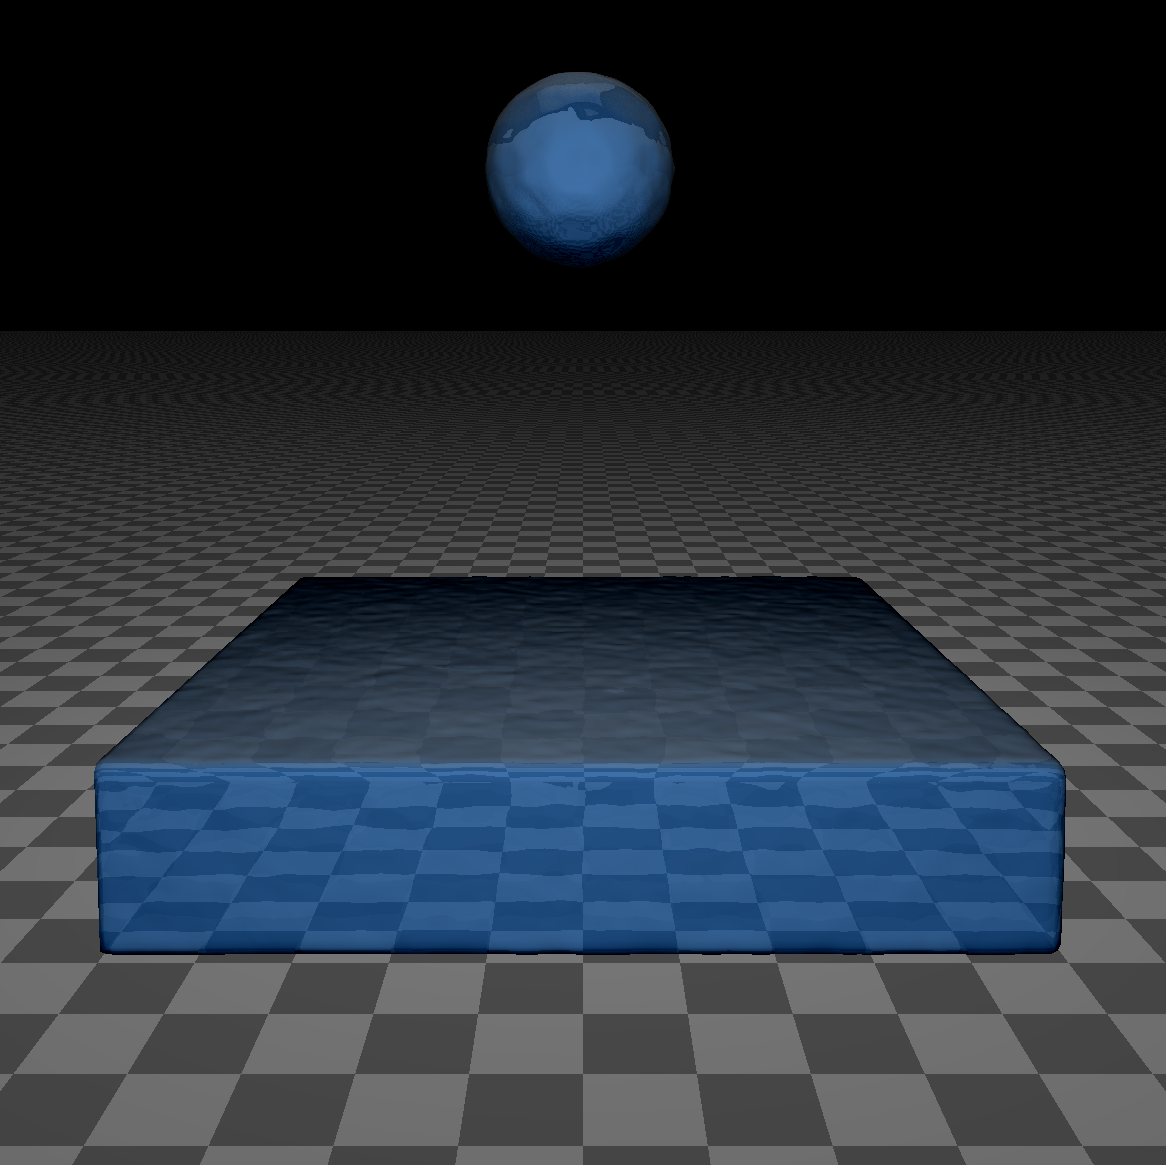
\includegraphics[width=6cm]{balldrop_cropped2/single0.png}
    \end{minipage}
    \begin{minipage}[t]{.42\linewidth}
        \centering
        \vspace{0pt}
        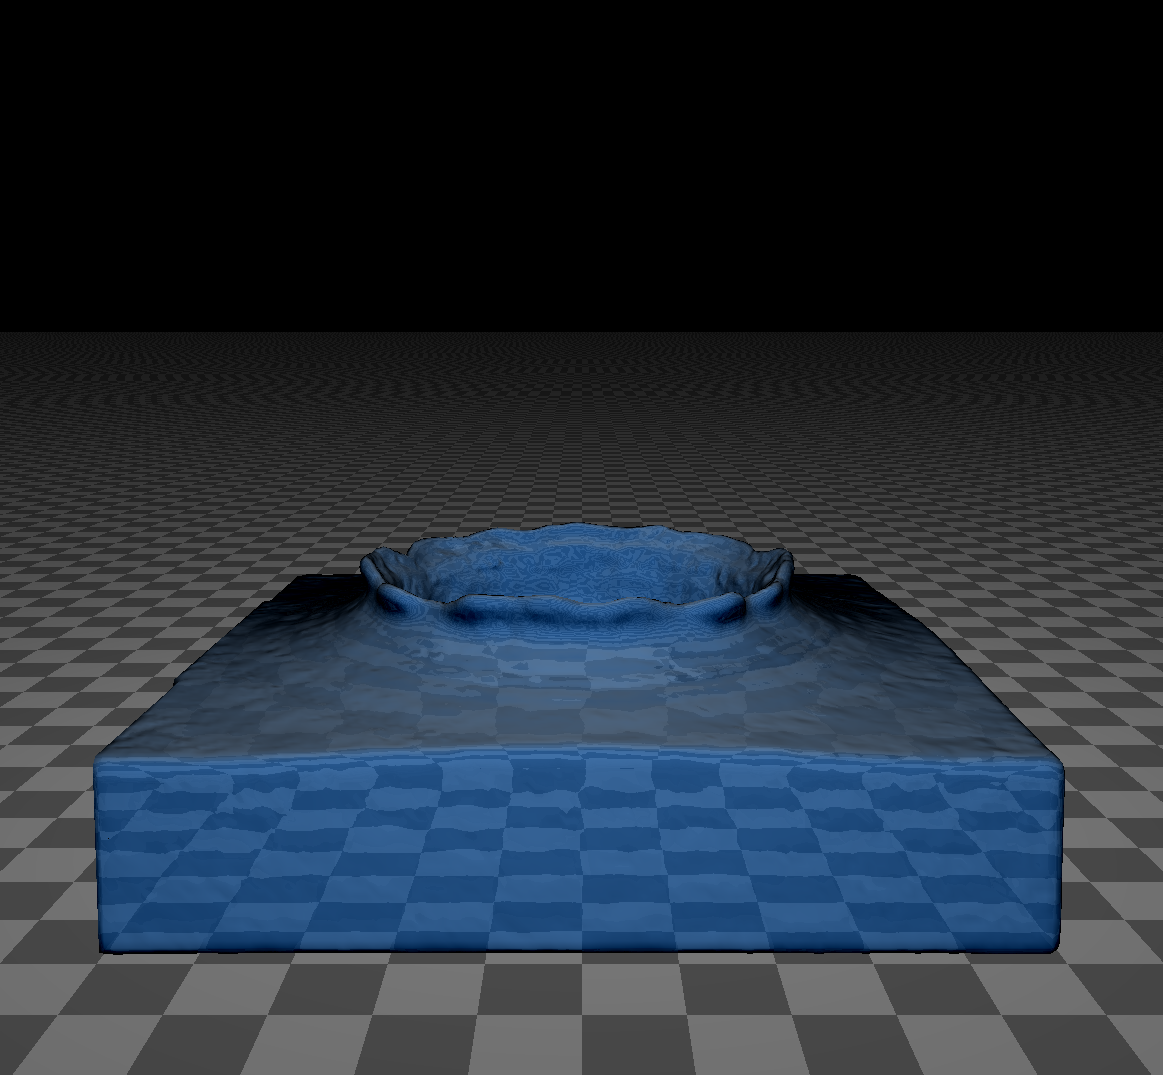
\includegraphics[width=6cm]{balldrop_cropped2/single1.png}
    \end{minipage}

    \vspace{0.5cm}

    \begin{minipage}[t]{.42\linewidth}
        \centering
        \vspace{0pt}
        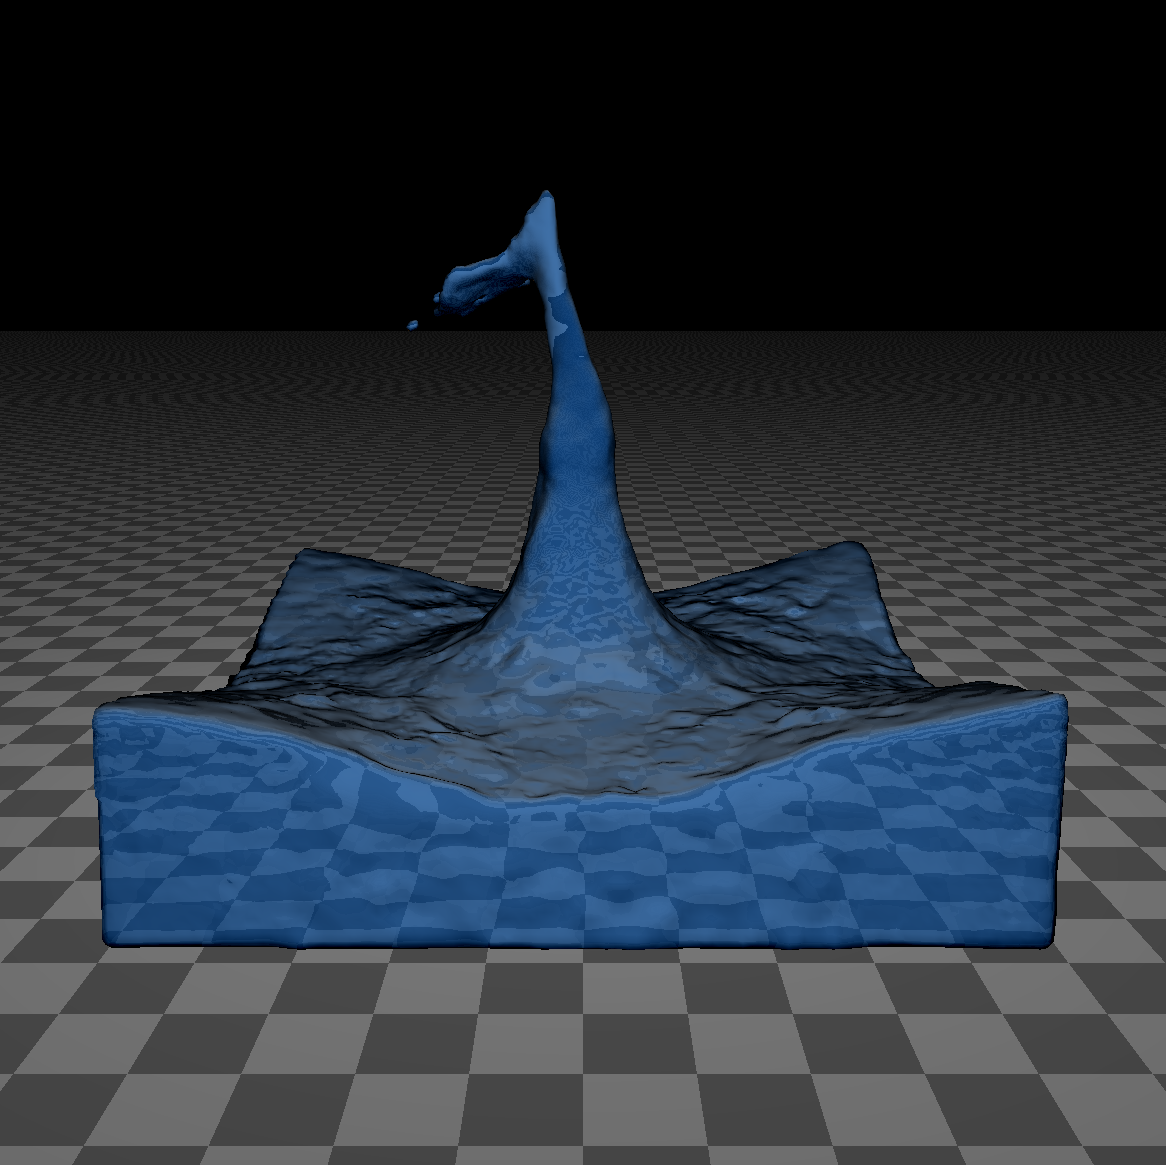
\includegraphics[width=6cm]{balldrop_cropped2/single2.png}
    \end{minipage}
    \begin{minipage}[t]{.42\linewidth}
        \centering
        \vspace{0pt}
        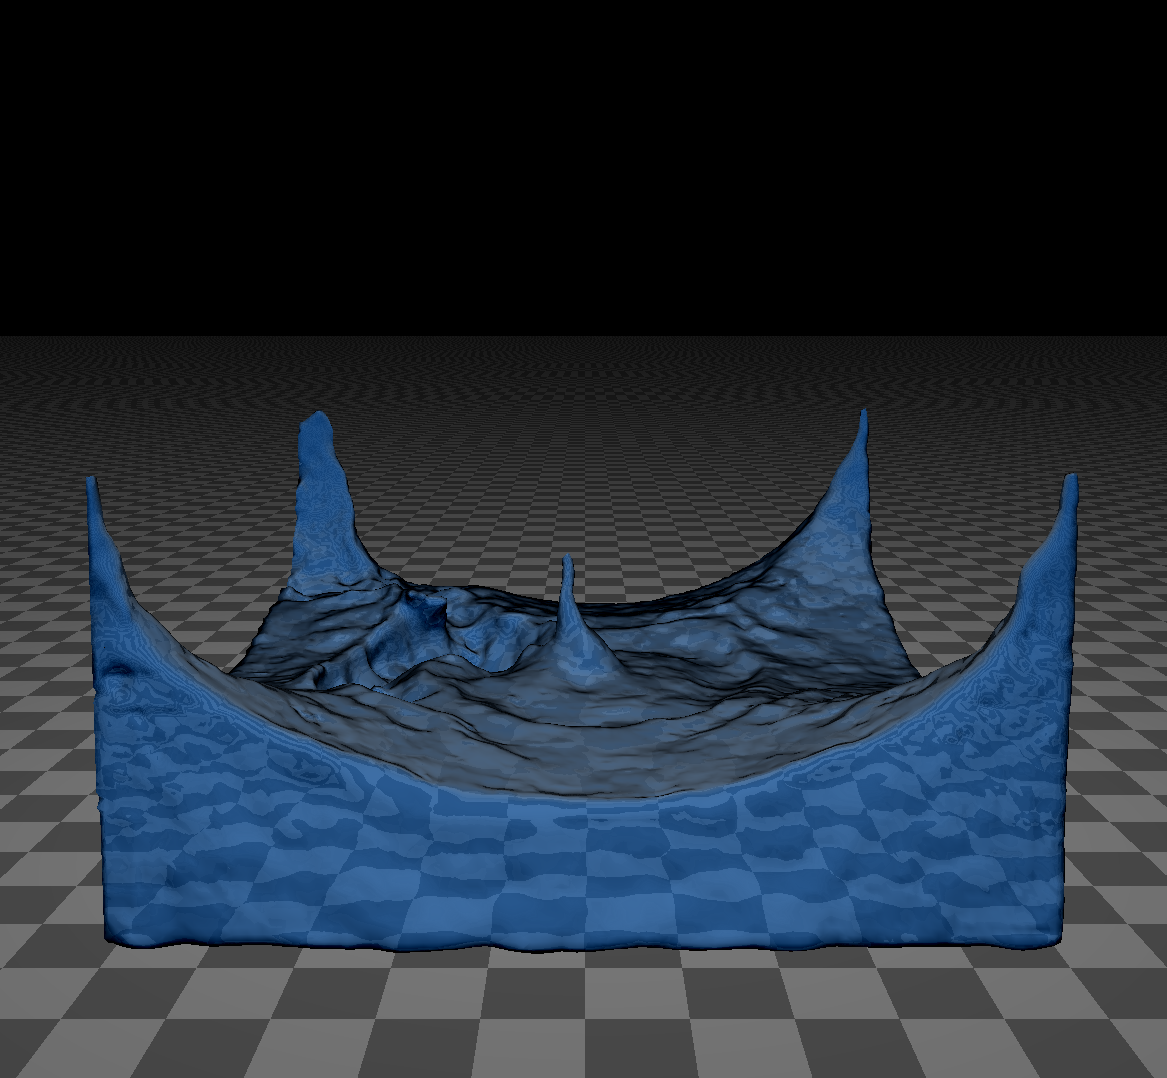
\includegraphics[width=6cm]{balldrop_cropped2/single3.png}
    \end{minipage}

    \caption{Ball drop. $50^3$ grid, $208k$ FLIP particles}
    \label{figure ball drop single}
\end{figure}


\begin{figure}[H]
    \centering
    
    \begin{minipage}[t]{.42\linewidth}
        \centering
        \vspace{0pt}
        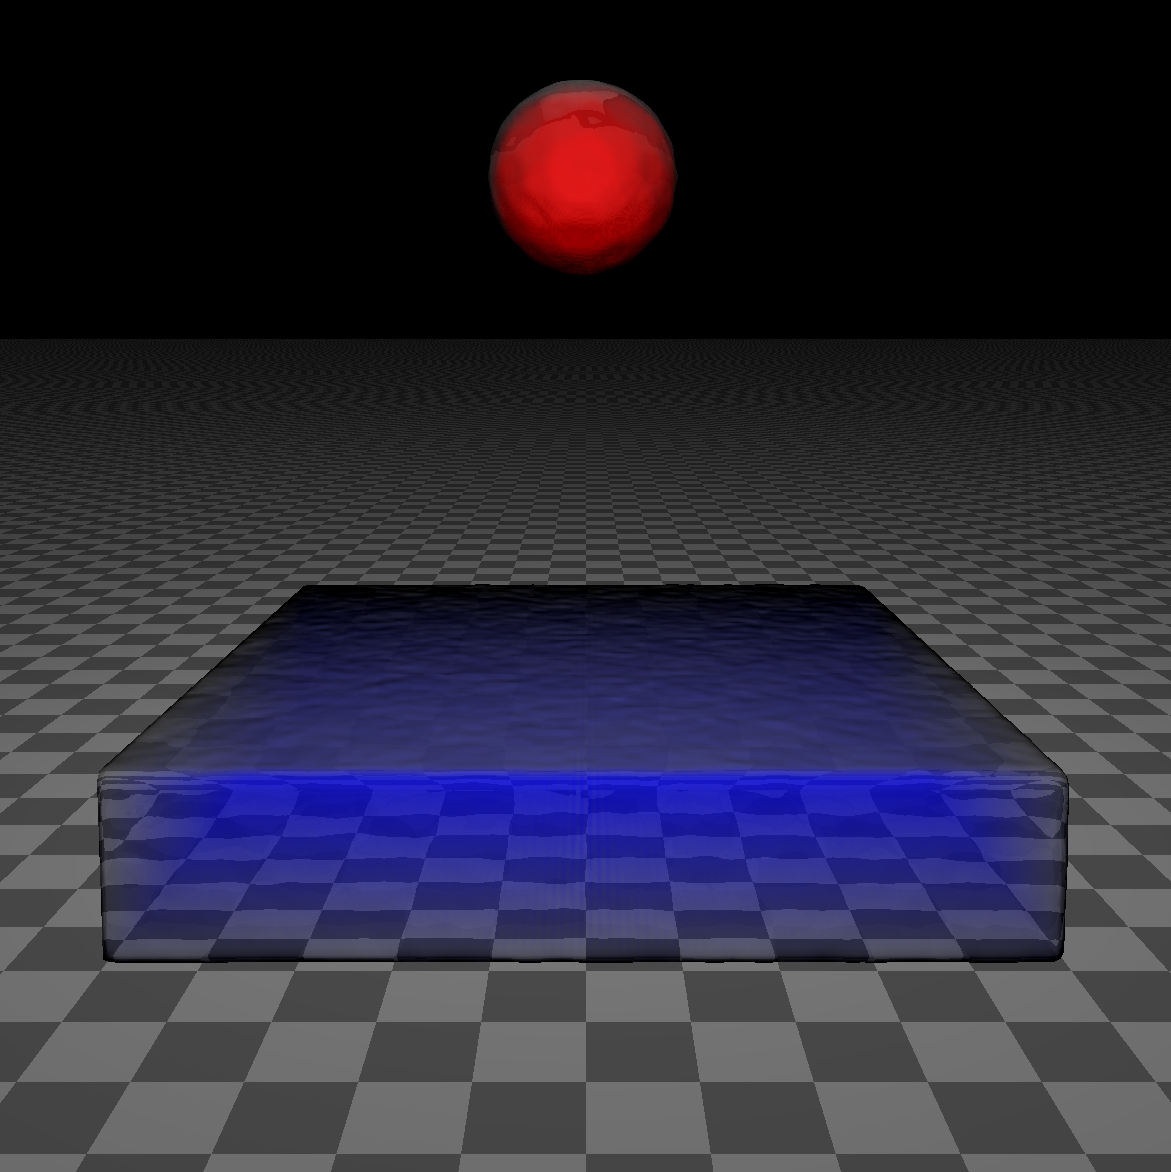
\includegraphics[width=6cm]{balldrop_cropped2/multi0.png}
    \end{minipage}
    \begin{minipage}[t]{.42\linewidth}
        \centering
        \vspace{0pt}
        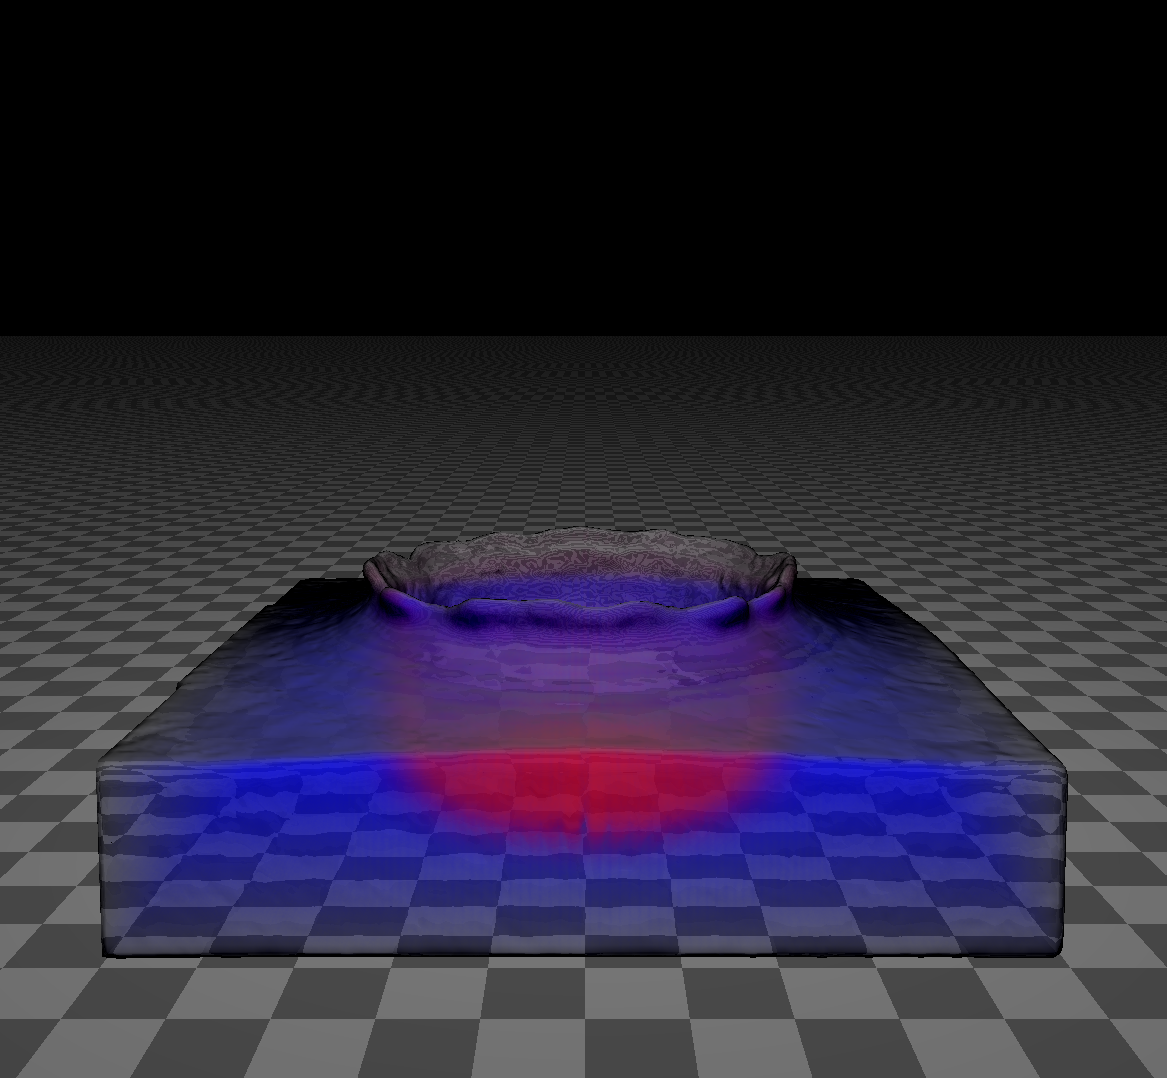
\includegraphics[width=6cm]{balldrop_cropped2/multi1.png}
    \end{minipage}

    \vspace{0.5cm}

    \begin{minipage}[t]{.42\linewidth}
        \centering
        \vspace{0pt}
        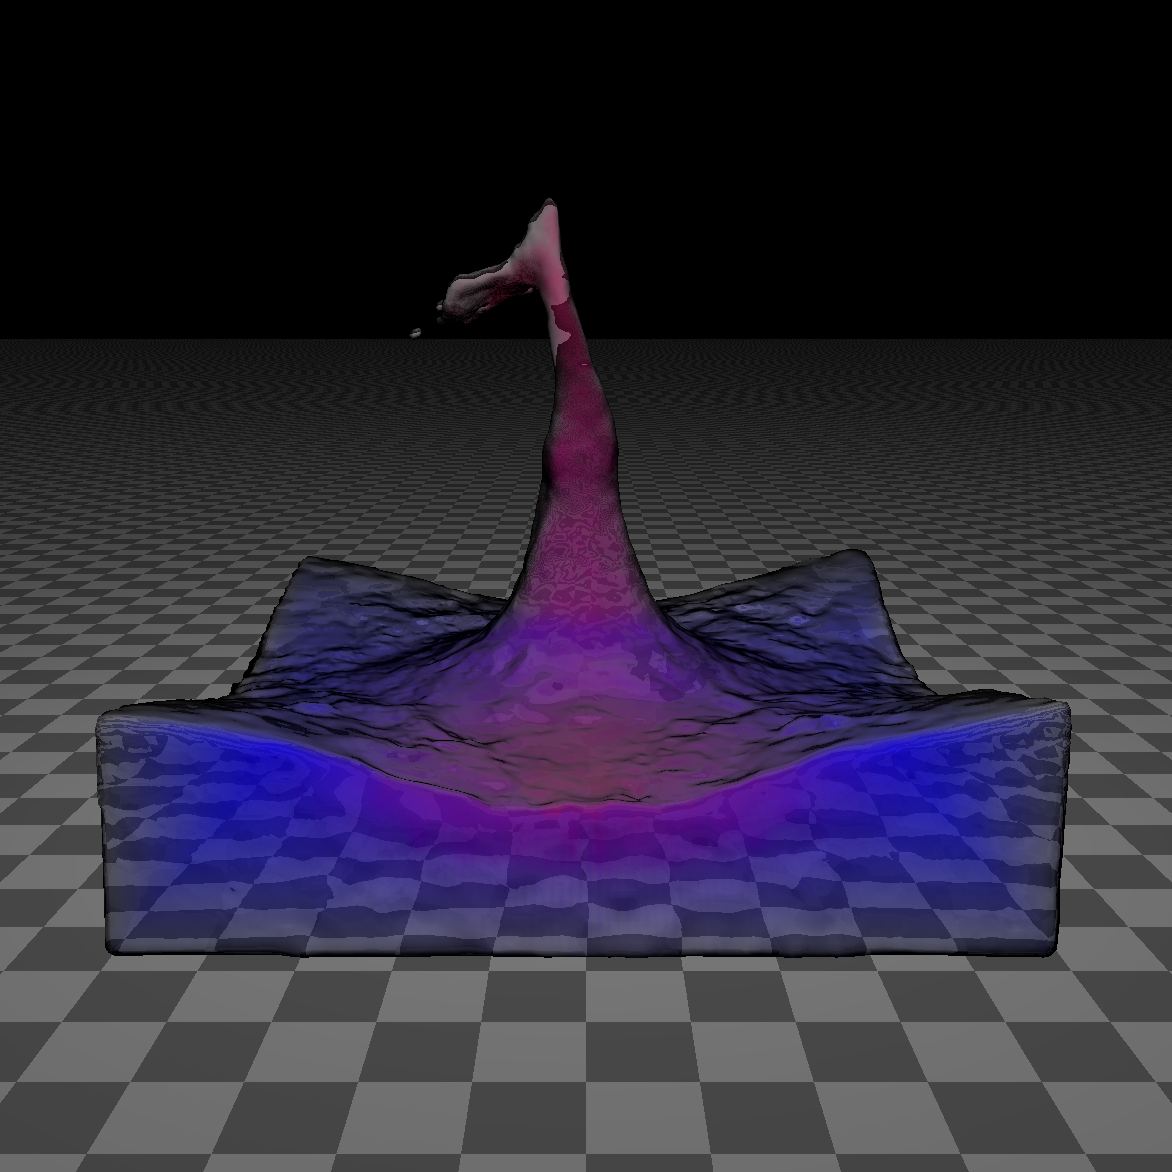
\includegraphics[width=6cm]{balldrop_cropped2/multi2.png}
    \end{minipage}
    \begin{minipage}[t]{.42\linewidth}
        \centering
        \vspace{0pt}
        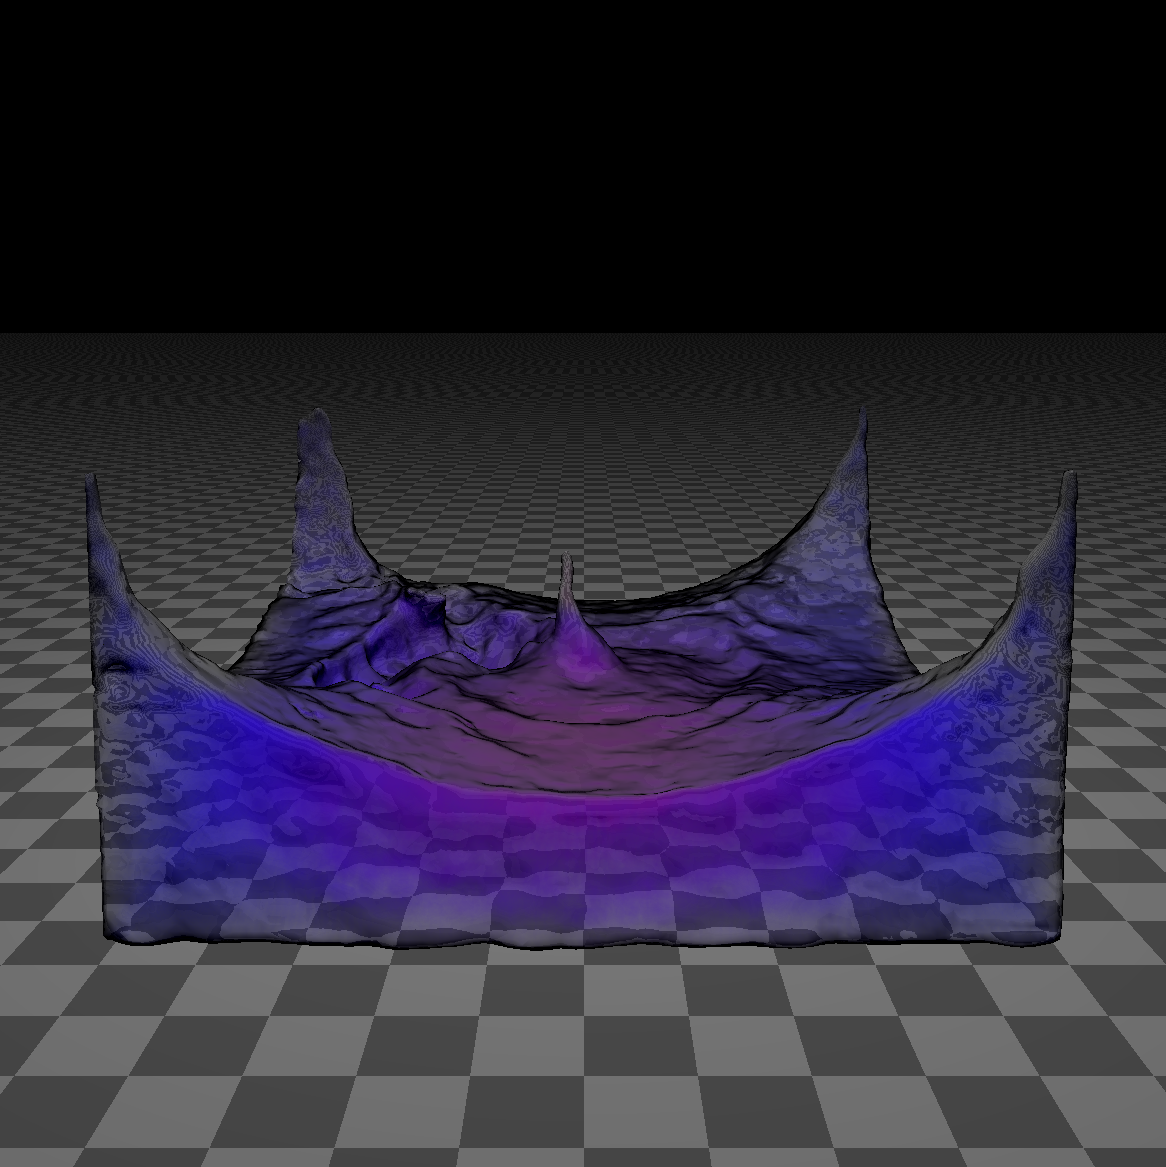
\includegraphics[width=6cm]{balldrop_cropped2/multi3.png}
    \end{minipage}

    \caption{Same simulation as figure \ref{figure ball drop single}, except with 2 phases}
    \label{figure ball drop multi}
\end{figure}


\begin{figure}[H]
    \centering
    
    \begin{minipage}[t]{.24\linewidth}
        \centering
        \vspace{0pt}
        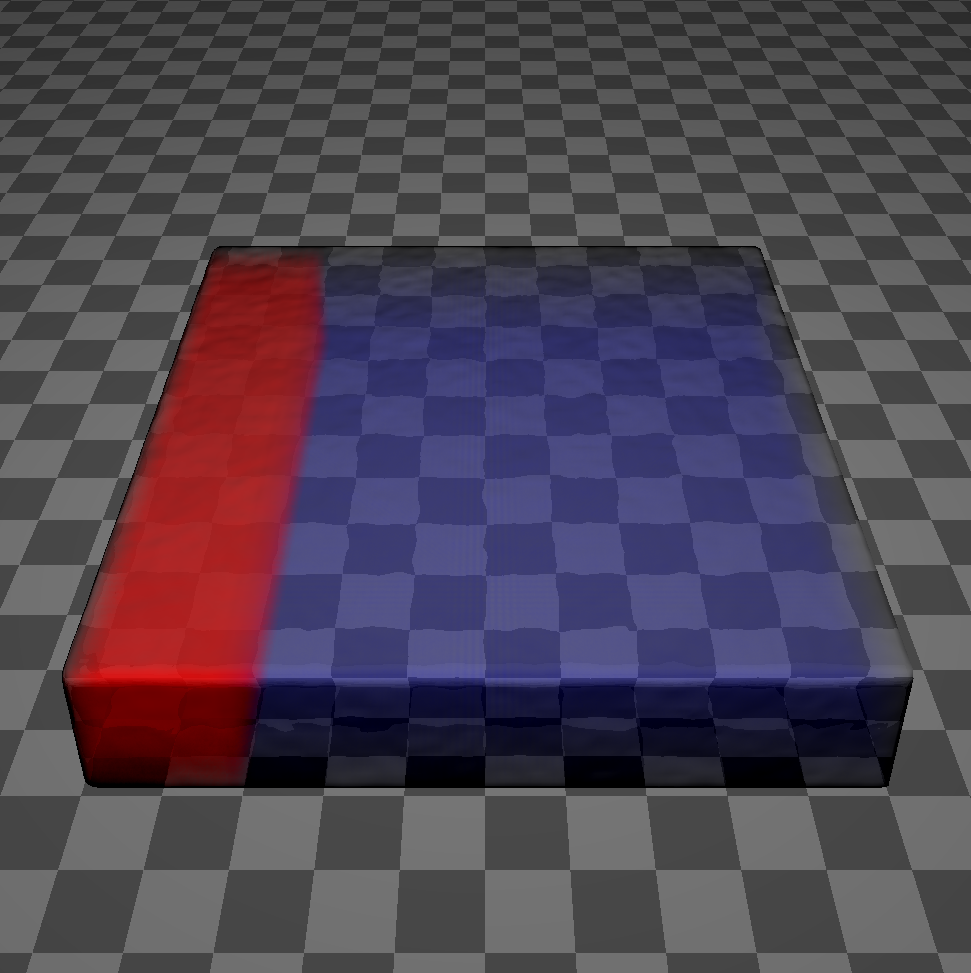
\includegraphics[width=3.5cm]{diffusion_cropped/small0.png}
    \end{minipage}
    \begin{minipage}[t]{.24\linewidth}
        \centering
        \vspace{0pt}
        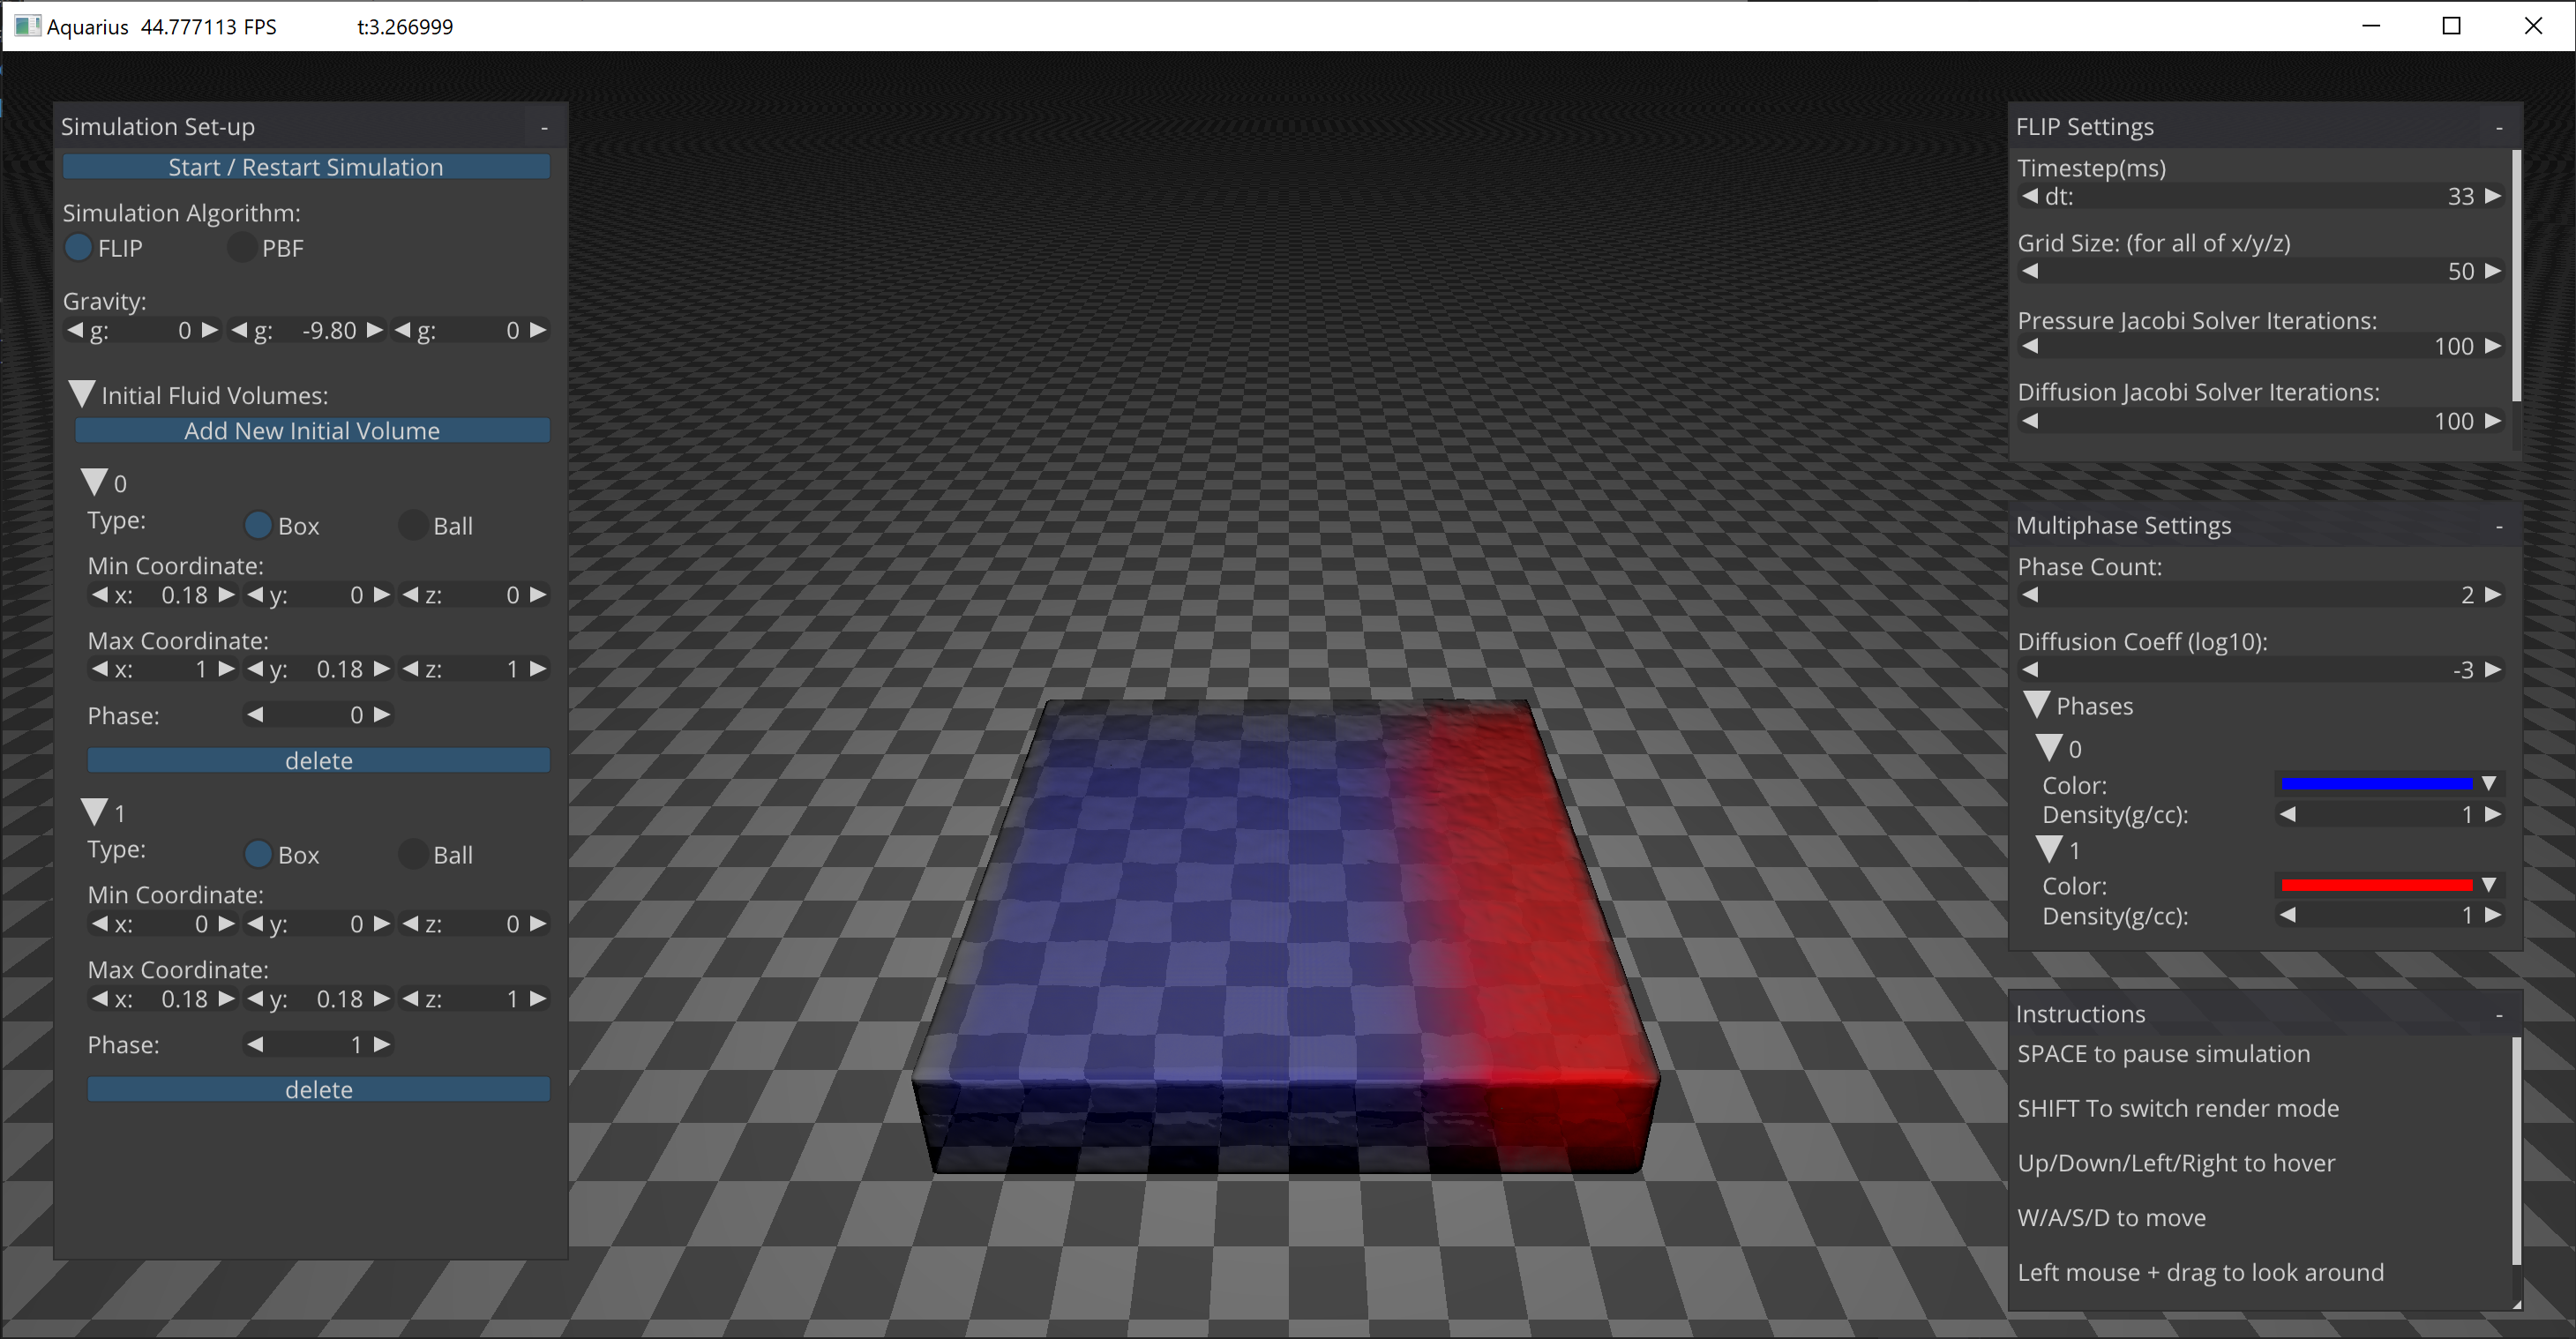
\includegraphics[width=3.5cm]{diffusion_cropped/small1.png}
    \end{minipage}
    \begin{minipage}[t]{.24\linewidth}
        \centering
        \vspace{0pt}
        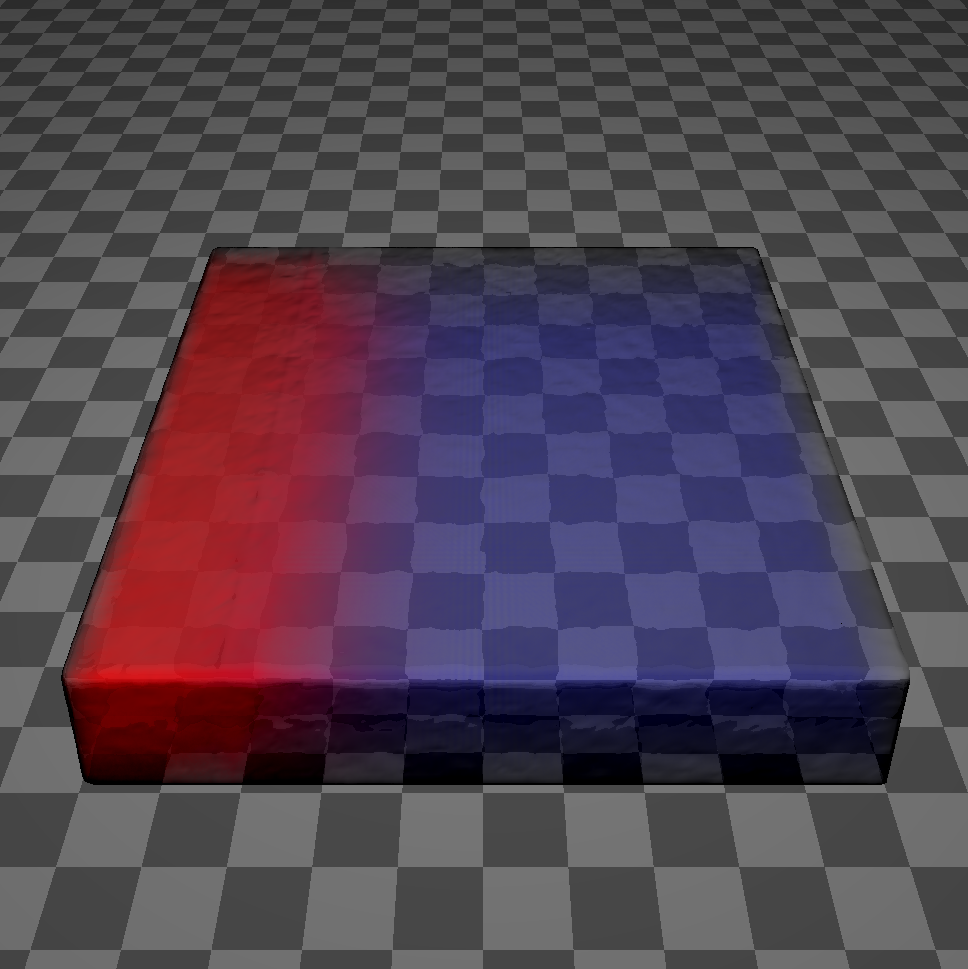
\includegraphics[width=3.5cm]{diffusion_cropped/small2.png}
    \end{minipage}
    \begin{minipage}[t]{.24\linewidth}
        \centering
        \vspace{0pt}
        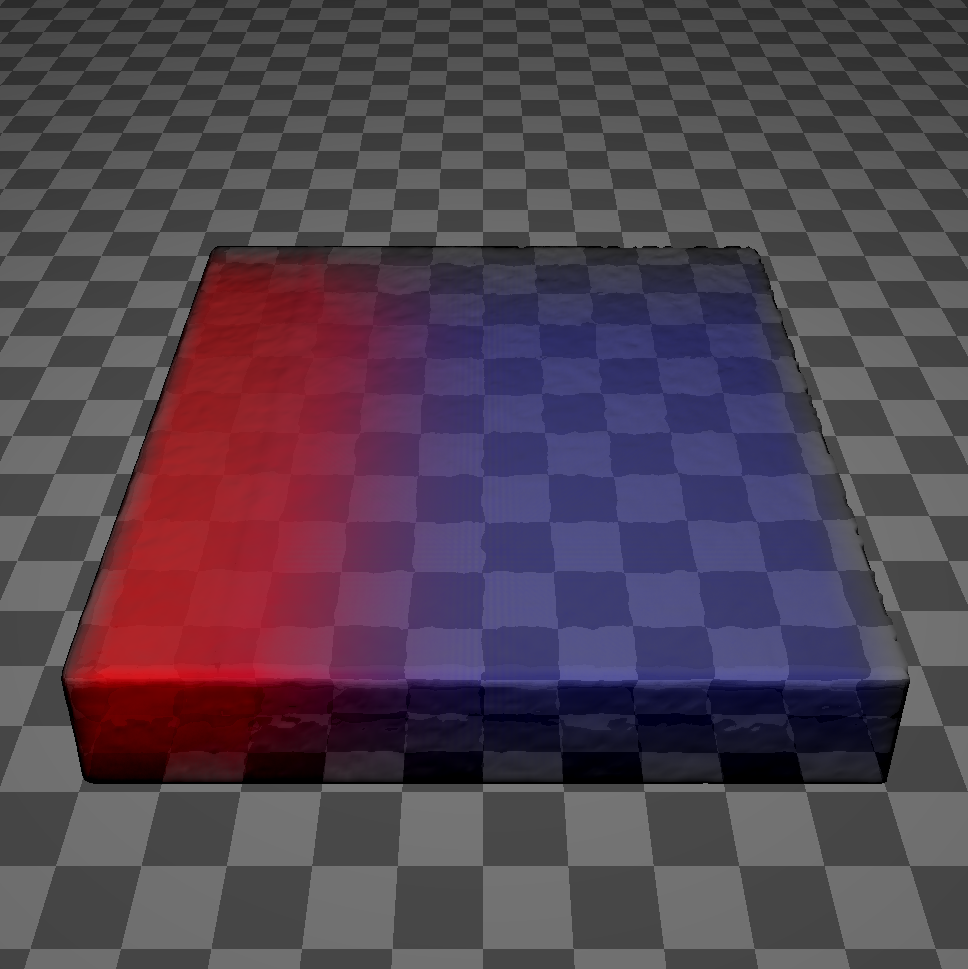
\includegraphics[width=3.5cm]{diffusion_cropped/small3.png}
    \end{minipage}

    \caption{Diffusion with coefficient $10^{-3}$}
    \label{diffusion 1e-3}
\end{figure}



\begin{figure}[H]
    \centering
    
    \begin{minipage}[t]{.24\linewidth}
        \centering
        \vspace{0pt}
        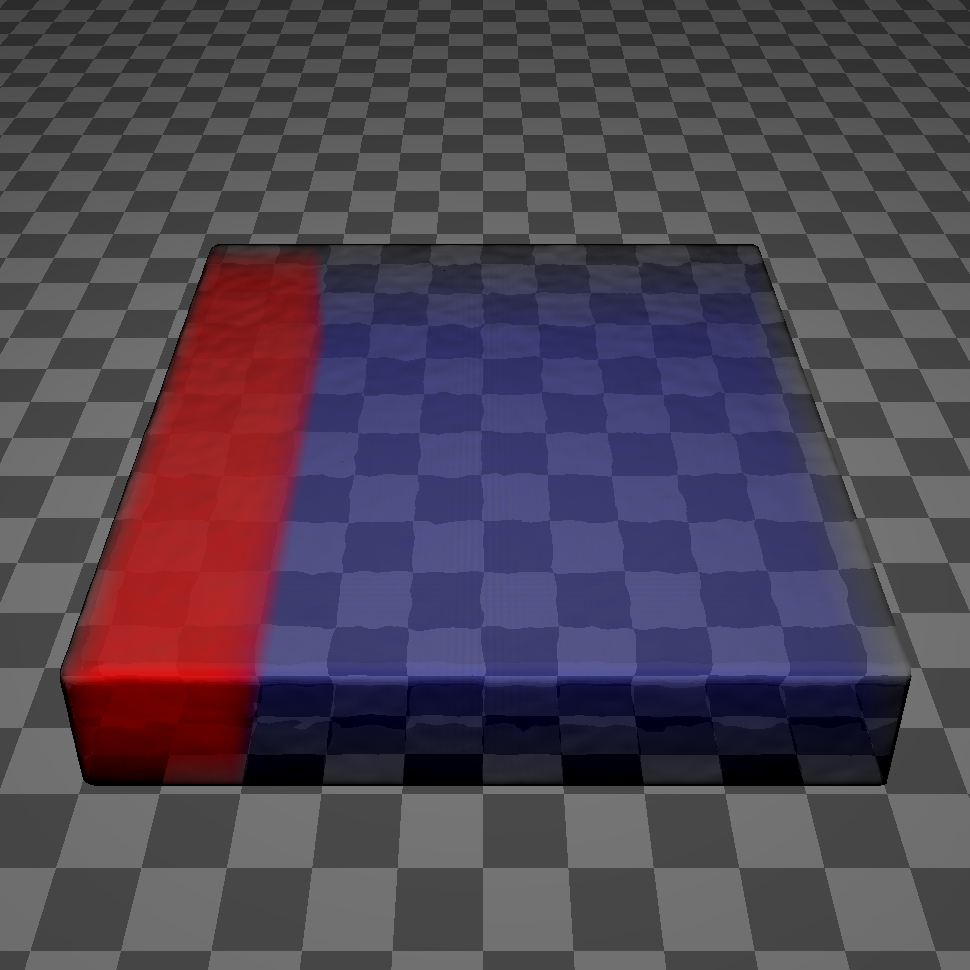
\includegraphics[width=3.5cm]{diffusion_cropped/big0.png}
    \end{minipage}
    \begin{minipage}[t]{.24\linewidth}
        \centering
        \vspace{0pt}
        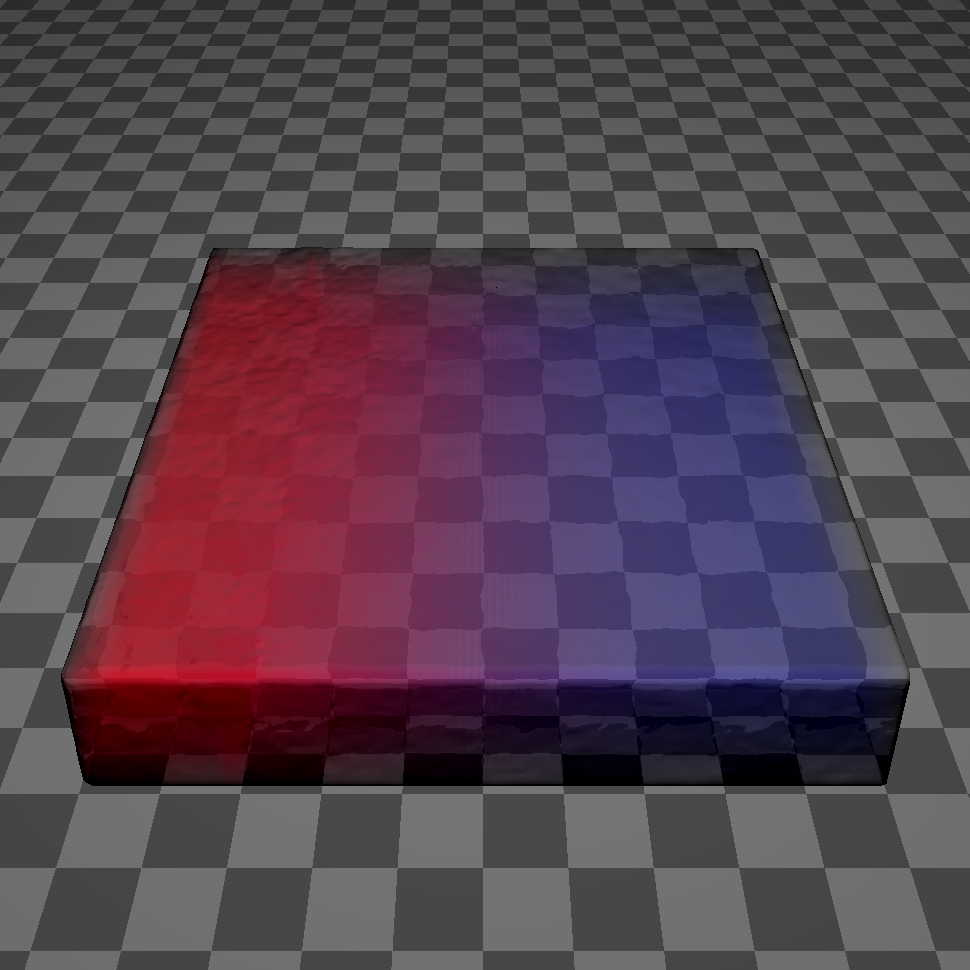
\includegraphics[width=3.5cm]{diffusion_cropped/big1.png}
    \end{minipage}
    \begin{minipage}[t]{.24\linewidth}
        \centering
        \vspace{0pt}
        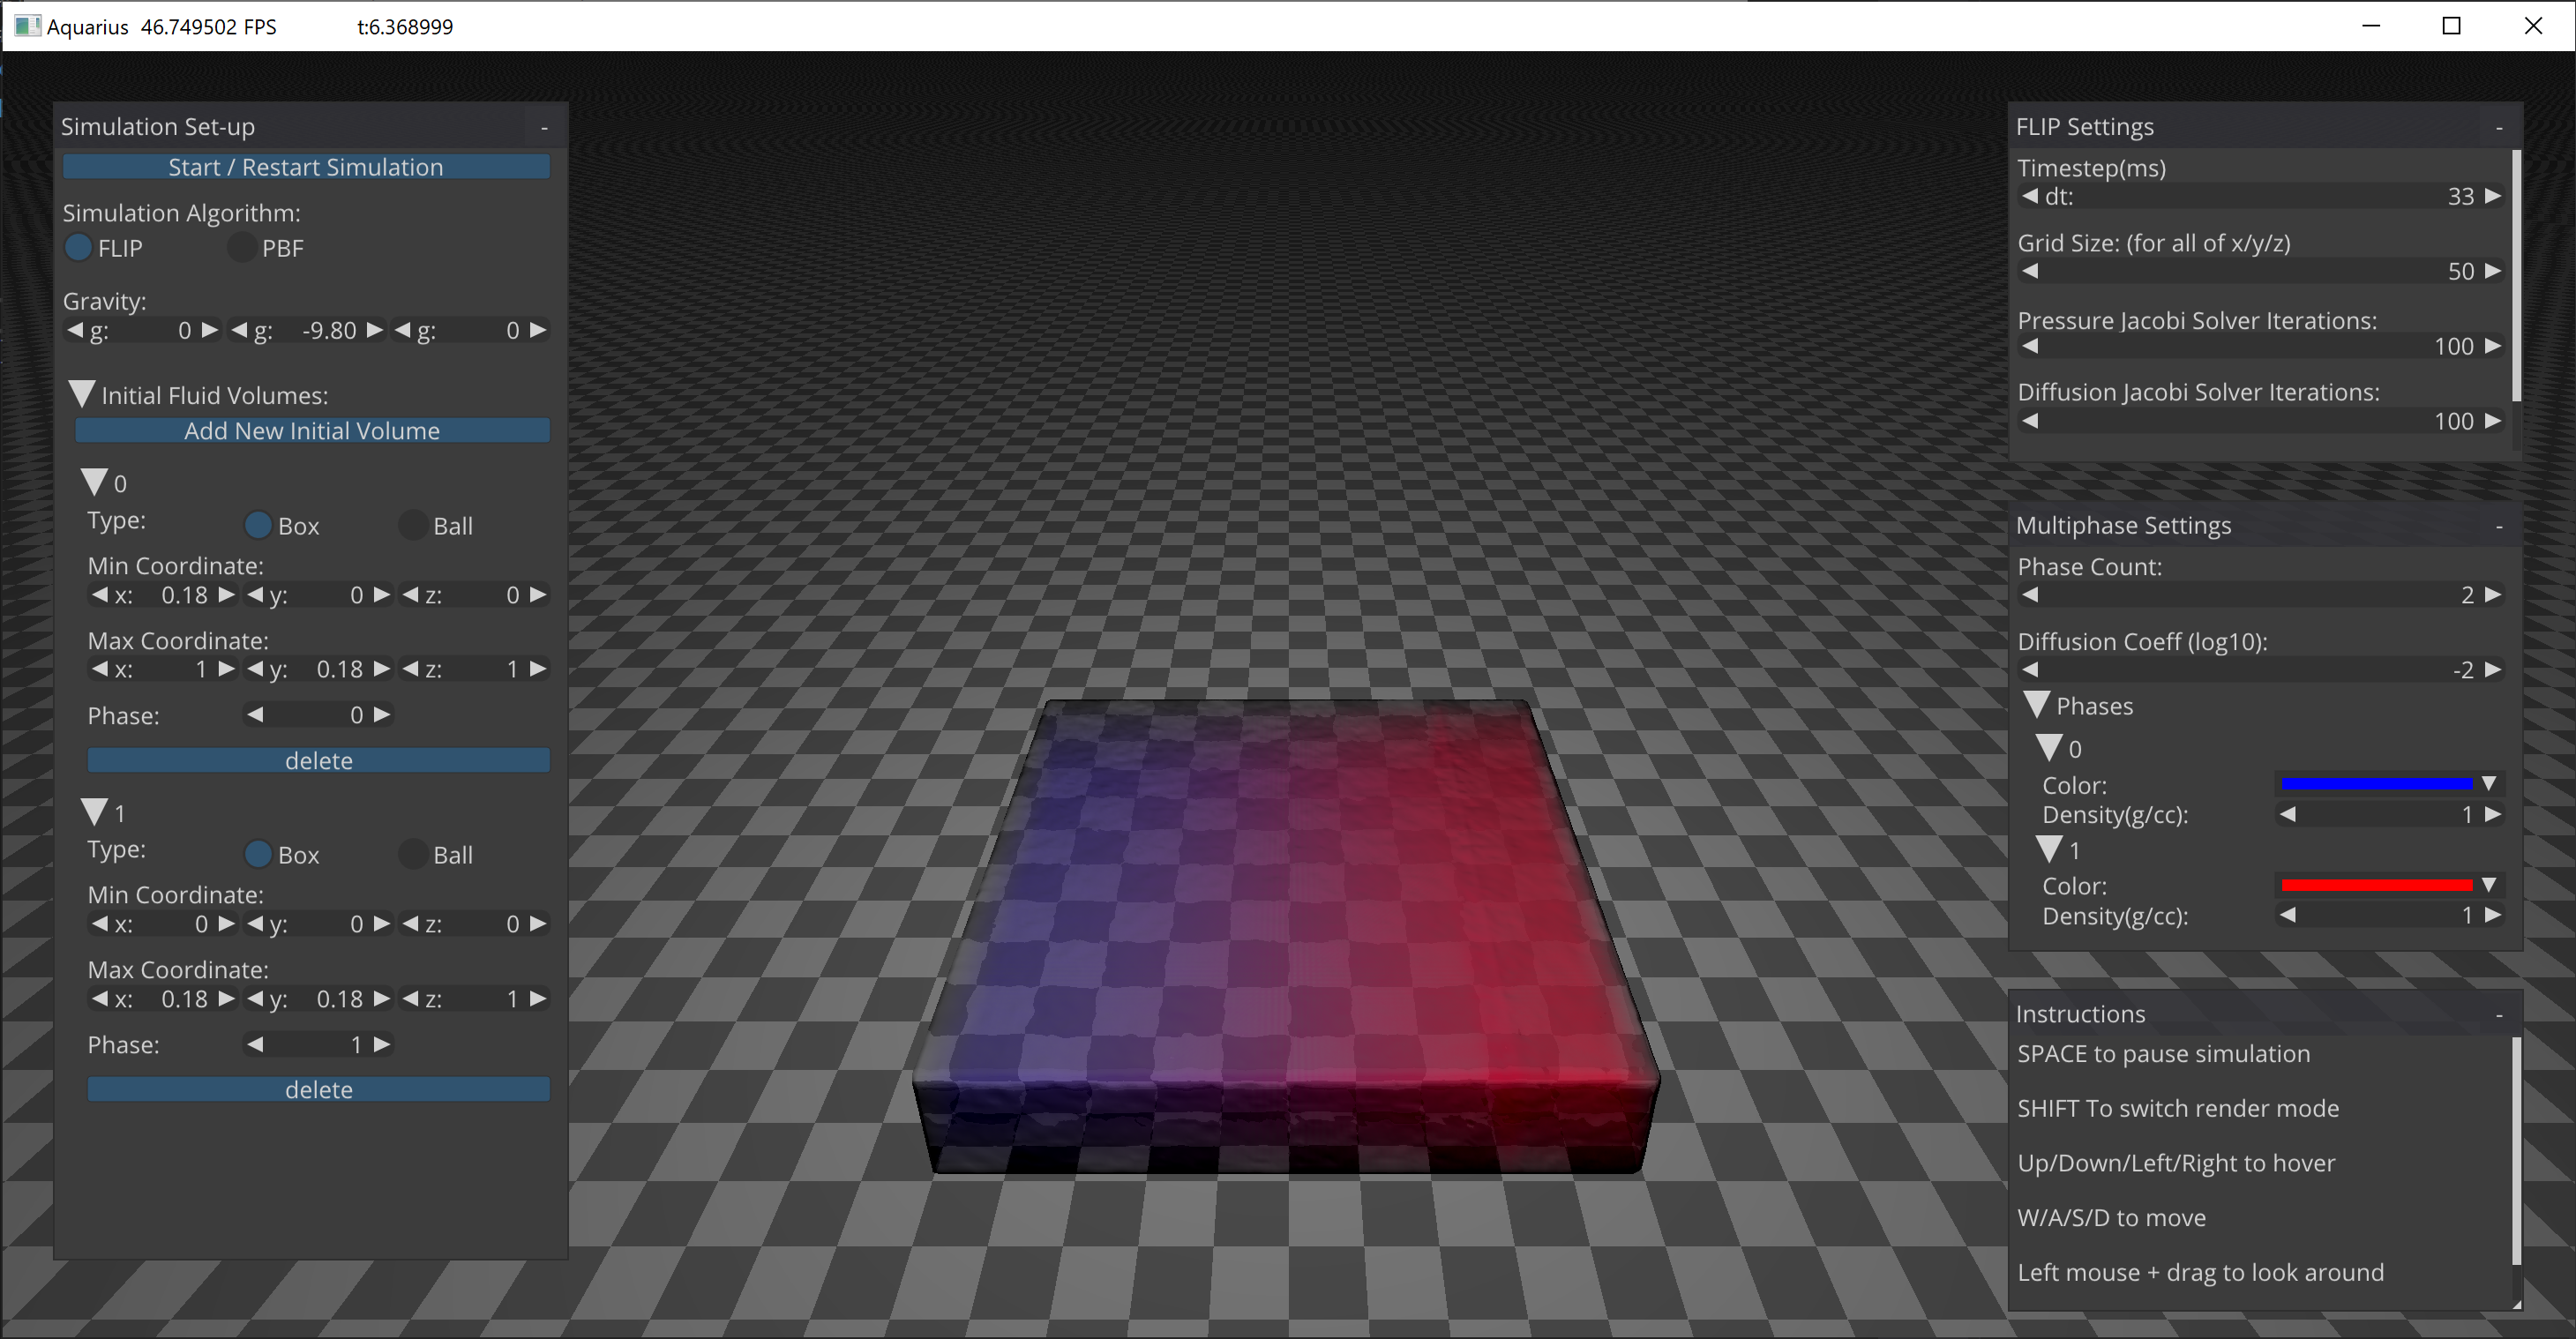
\includegraphics[width=3.5cm]{diffusion_cropped/big2.png}
    \end{minipage}
    \begin{minipage}[t]{.24\linewidth}
        \centering
        \vspace{0pt}
        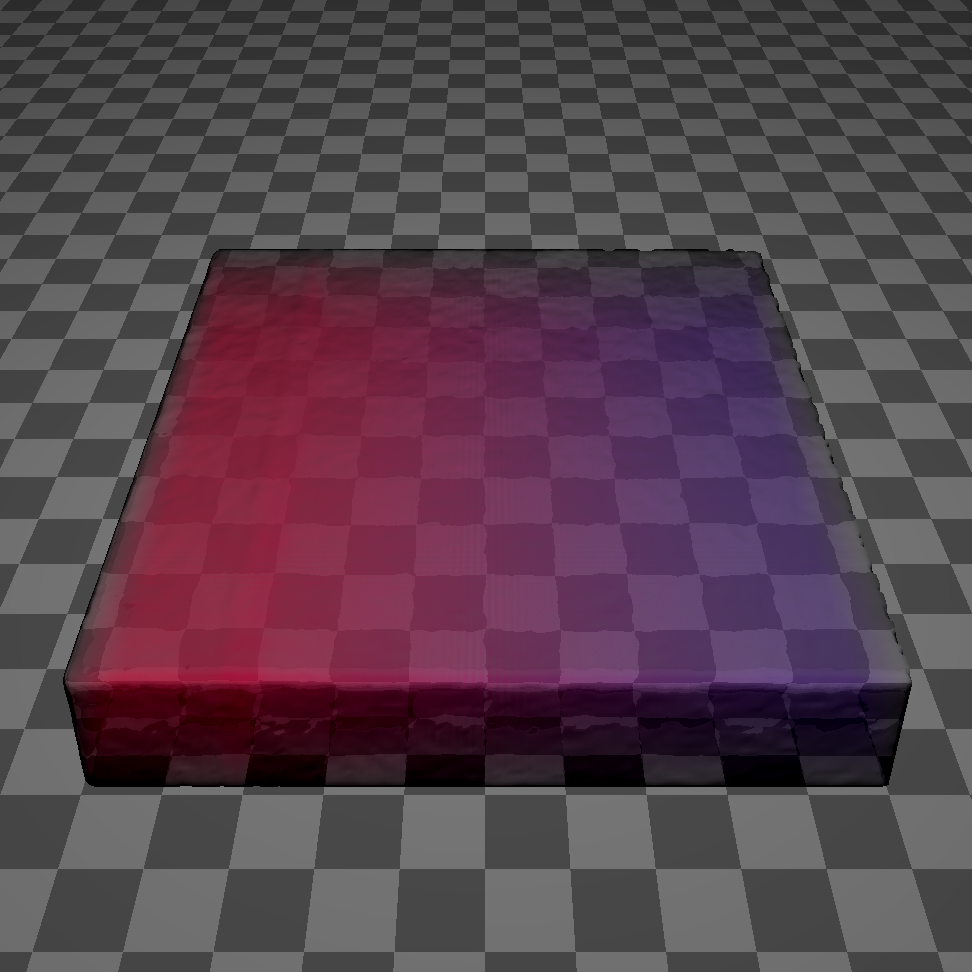
\includegraphics[width=3.5cm]{diffusion_cropped/big3.png}
    \end{minipage}

    \caption{Diffusion with coefficient $10^{-2}$}
    \label{diffusion 1e-2}
\end{figure}

